\begin{figure}
\centering
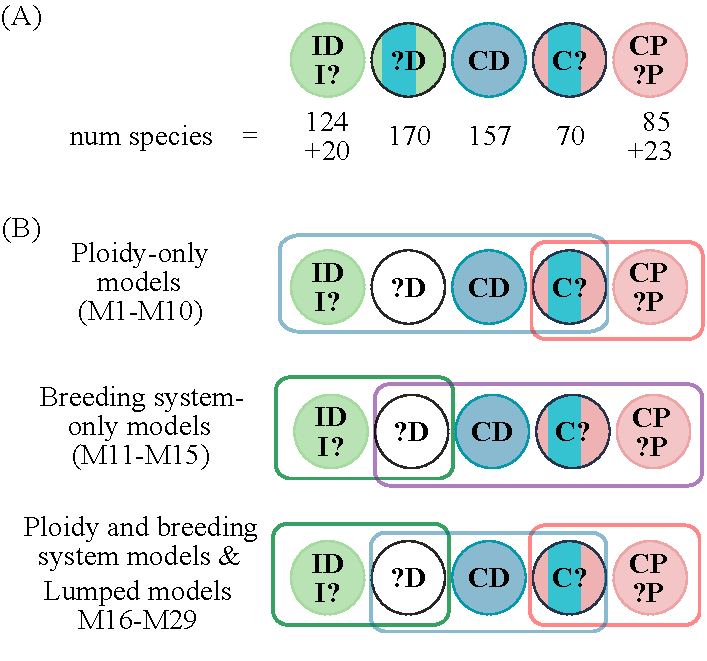
\includegraphics[width=0.5\textwidth]{fig1.pdf}
\caption{
Character states used in the models.
(A) Each species retained on the phylogeny belonged to one of five possible categories, depending on whether ploidy and/or breeding system were known. 
Number of species in each category is indicated; for example, 70 species are self-compatible with unknown ploidy.
Character state abbreviations are: $I$ for self-incompatible, $C$ for self-compatible, $D$ for diploid, $P$ for polyploid, $?$ for unknown.
Because polyploidization breaks this form of self-incompatibility, self-incompatible species with unobserved ploidy ($I?$) are taken to be diploid ($ID$), and polyploid species with unobserved breeding system ($?P$) are taken to be SC ($CP$).
(B) Category groupings into states for each model class.
In the ploidy-only models (M1- M10), states are coded as $D$ \& $P$ when uncertain/consistent with either state; in the breeding system-only models (M11-M15) such states are coded as $C$; in the ploidy and breeding system models (M16-M29), they are coded as $CD$ \& $CP$.
In the hidden-trait models, all species could take on either of two `hidden' character states. %IM: #33 
Two species, \emph{Lycium californicum} and \emph{Solanum bulbocastanum}, are simultaneously $ID$ and $CP$, and by adding them the sample adds to the total of 651 taxa used for analyses.
}\label{figure:stateclassifications}
\end{figure}

\begin{figure}
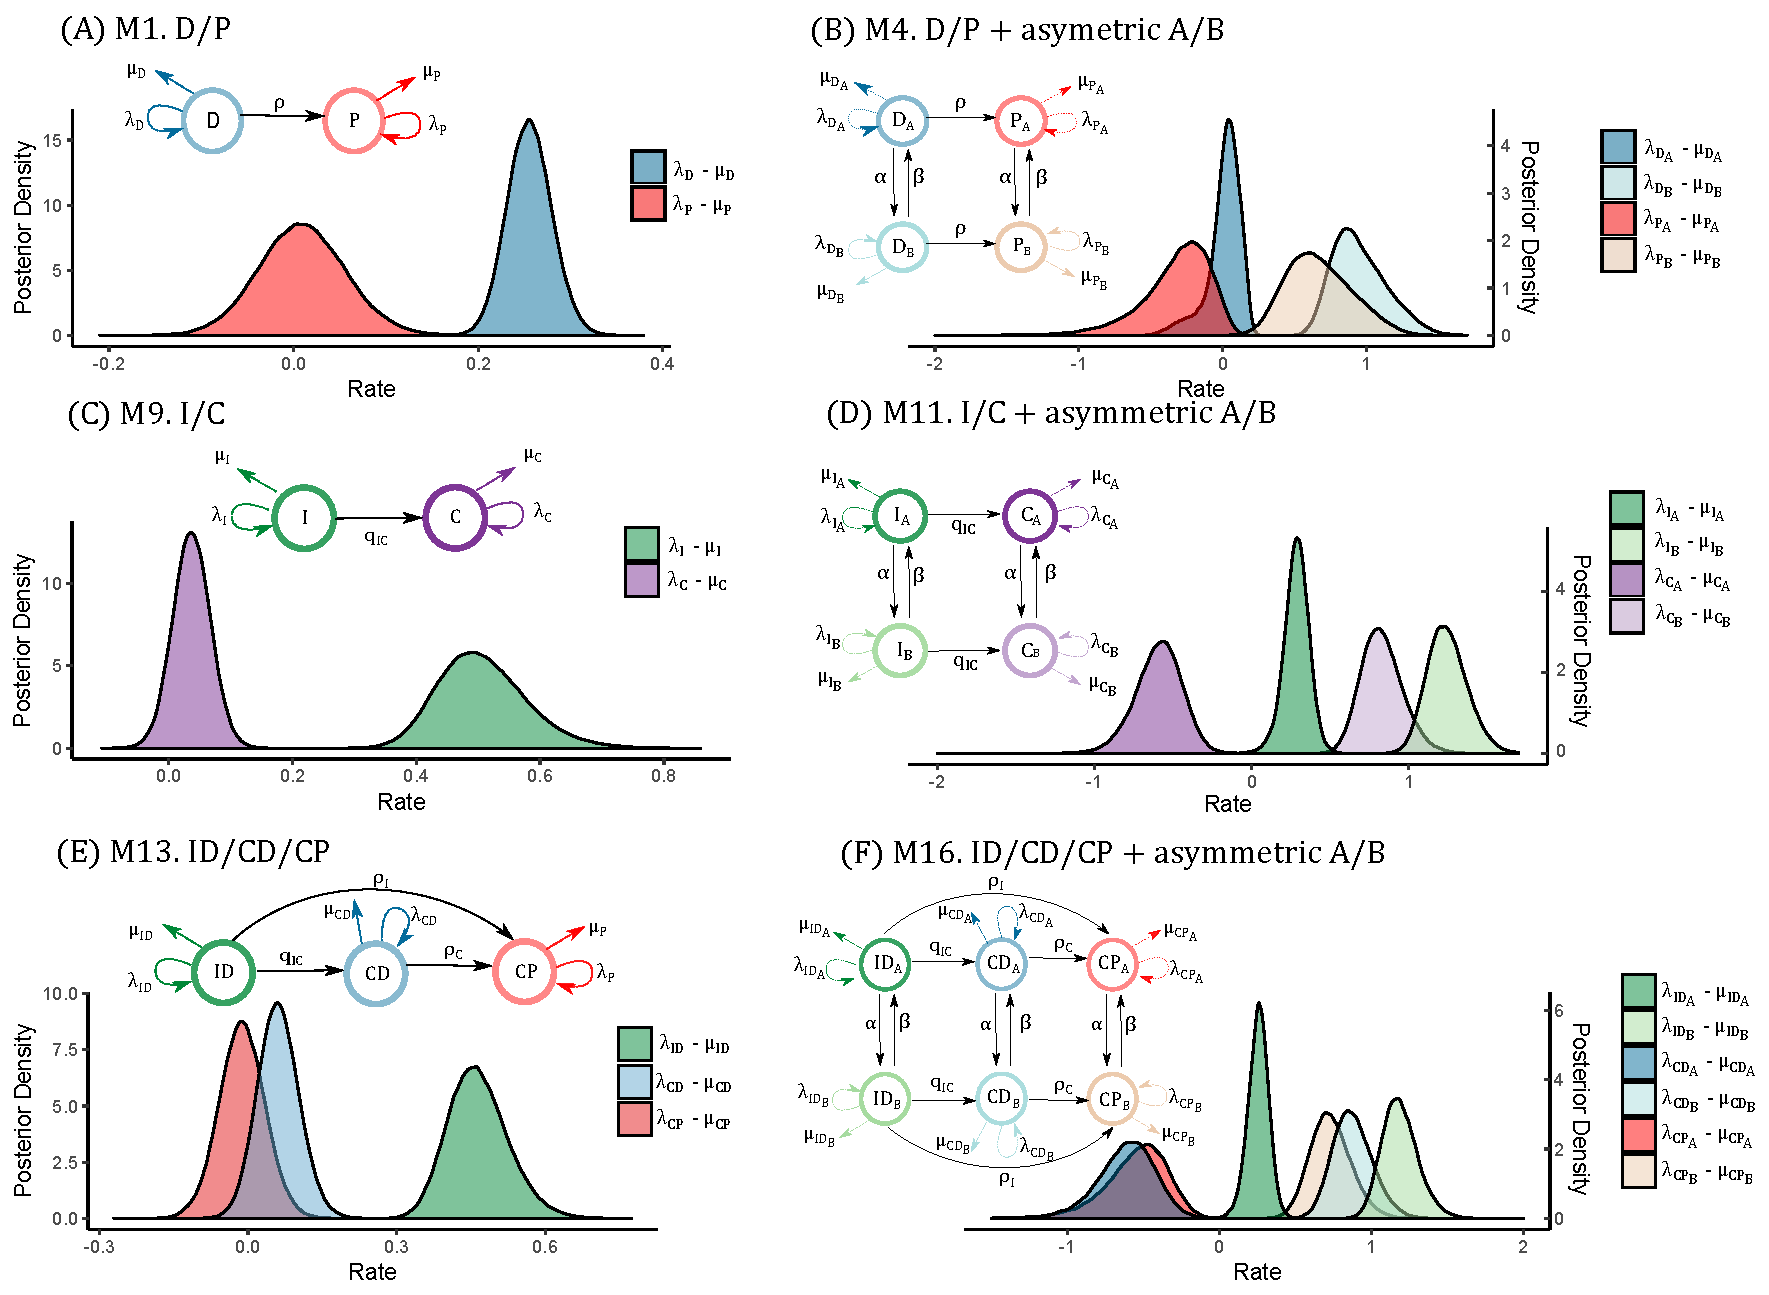
\includegraphics[width=\textwidth]{fig2.pdf} 
\caption{Net diversification rates for SSE models of focal traits with or without hidden state. 
(A) Ploidy only model (M1) showing higher net diversification linked to diploid state $D$ compared to polyploid state $P$.
(B) Ploidy with hidden states model (M4) showing that the net diversification is higher for hidden state $B$ (lighter colors) compared to hidden state $A$ (darker colors) and both diploid and polyploid states within each hidden traits have overlapping net diversification rates.
(C) Breeding system only model (M9) showing higher net diversification linked to self-incompatible $I$ state compared to self-compatible state $C$.
(D) Breeding system with hidden states model (M11) showing diversification differences in both hidden states (light \vs. dark colors) and little to no overlapping in between self-compatible \vs self-compatible states.
(E) Ploidy and breeding system model (M13) showing higher net diversification linked to self-incompatible diploid state $ID$ compared to both self-compatible states despite ploidy level ($CD, CP$).
(F) Ploidy, breeding system, and hidden states model (M16) showing a similar pattern that panel (E) within each hidden state $A$ and $B$. For hidden state $B$ there is a larger overlap of net diversification between states $CD_B$ and $ID_B$.}
\label{figure:netdivall}
\end{figure}

\begin{figure}
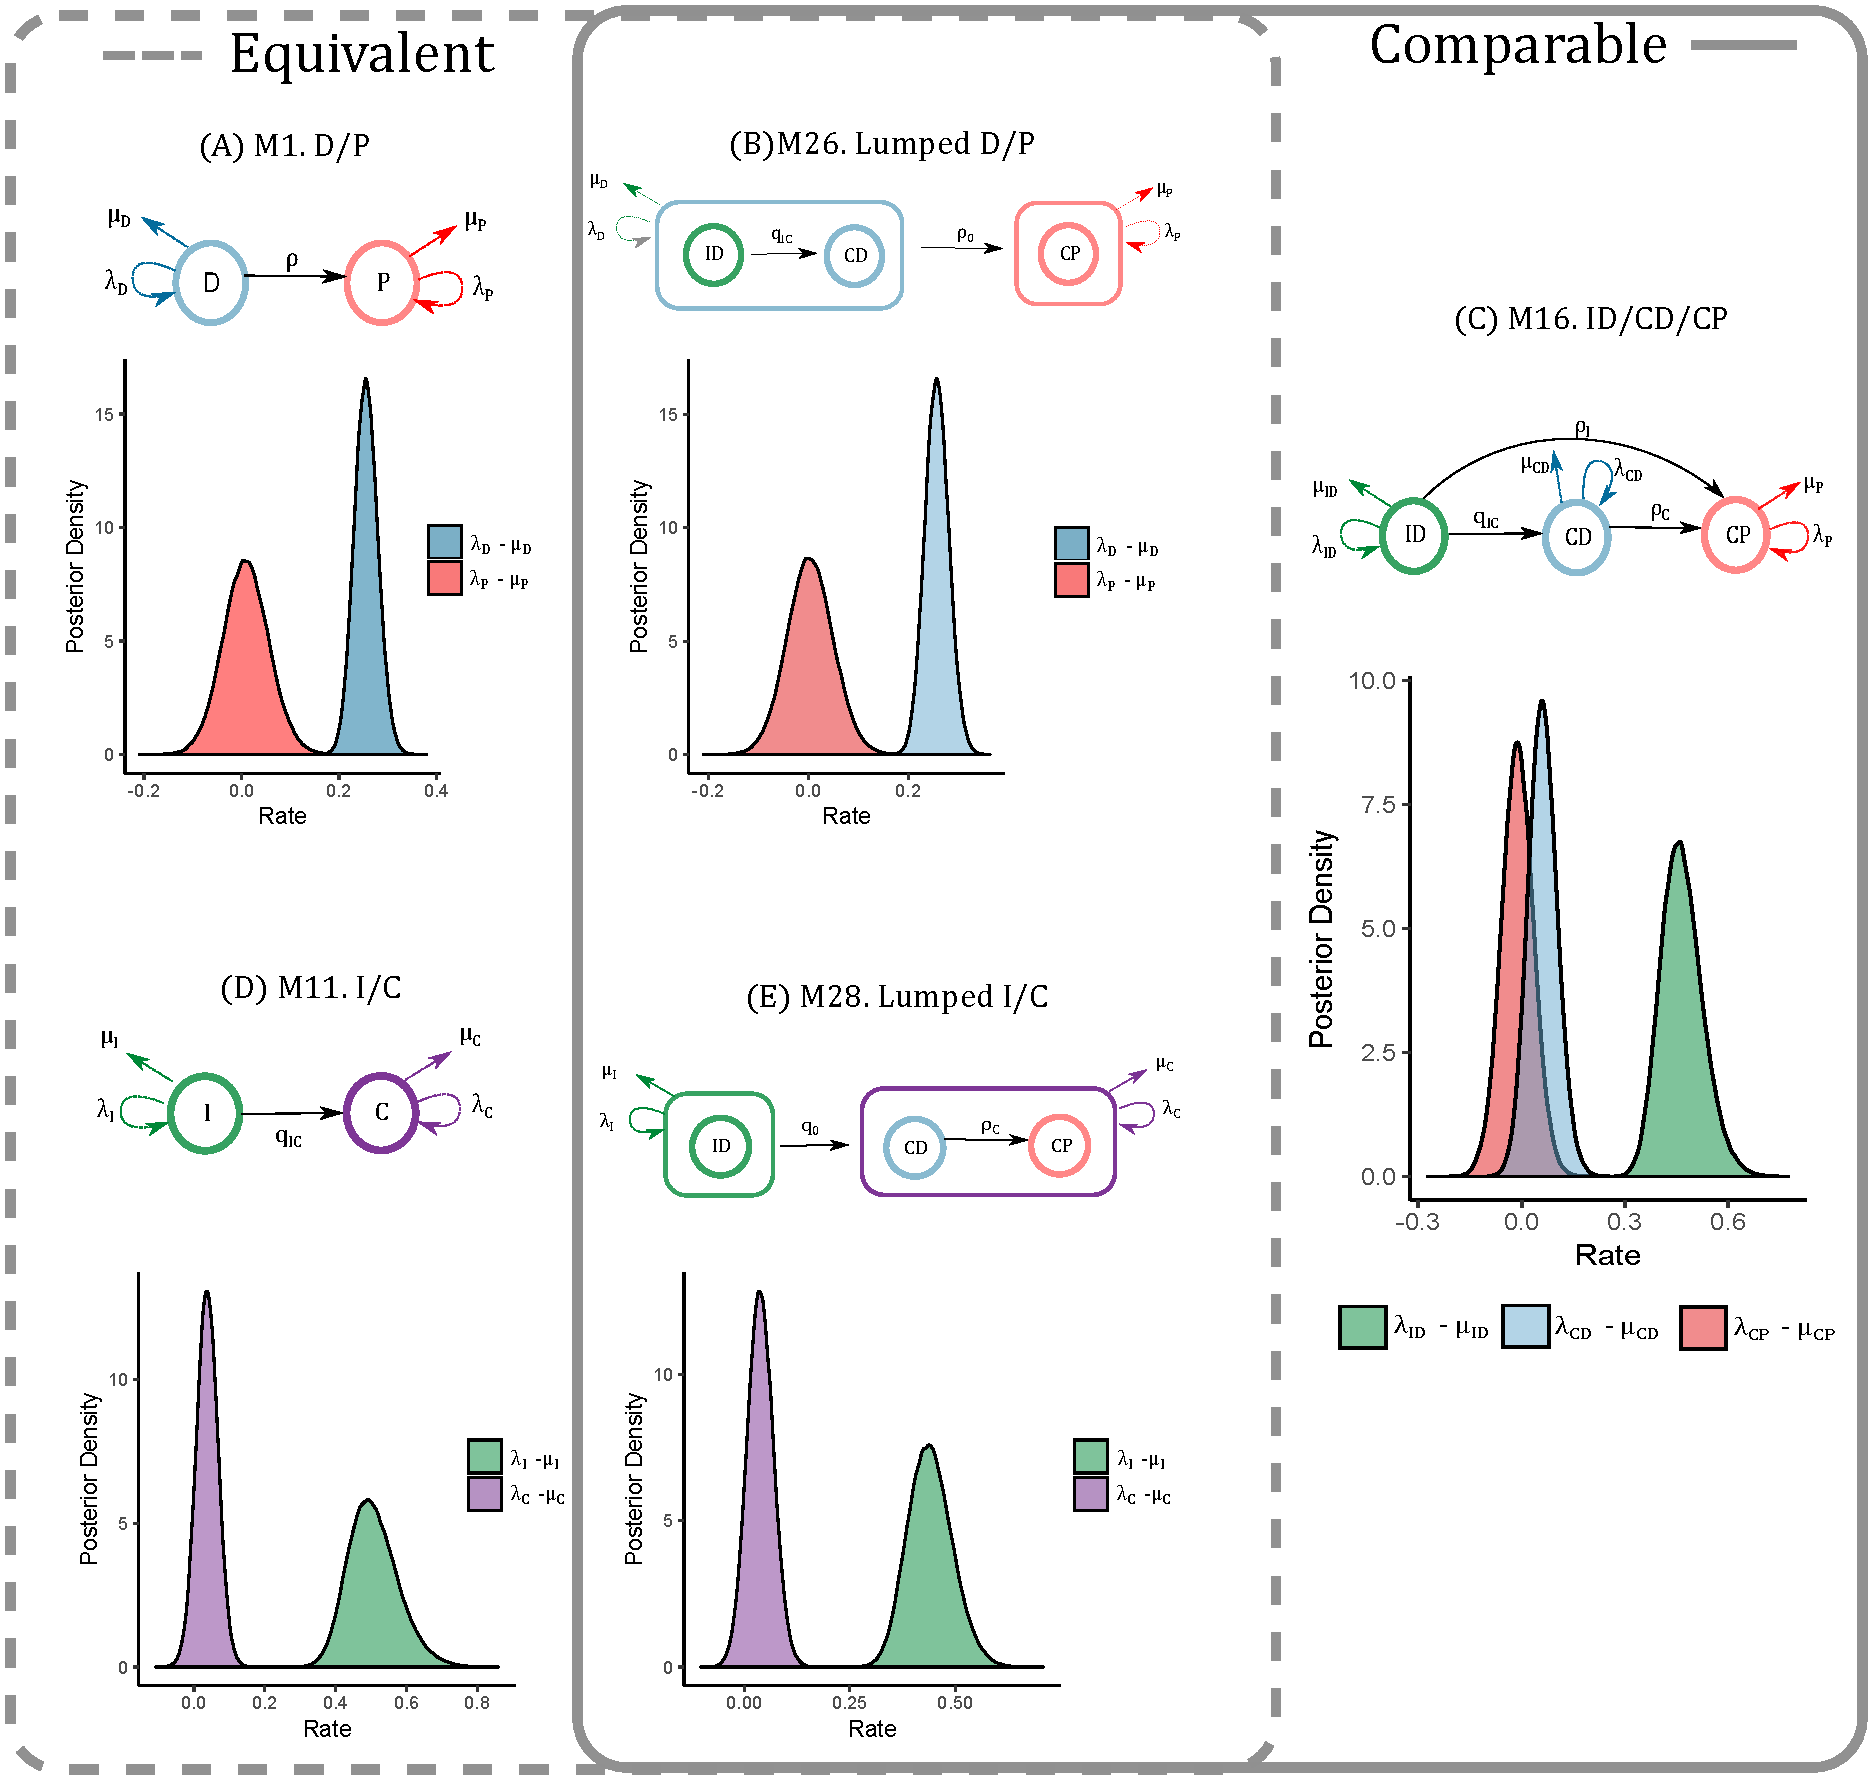
\includegraphics[width=\textwidth]{fig3.pdf} %lumped.pdf
\caption{Comparing two and three-state models using lumped models. (A) Ploidy model only (M1) where data enter as binary $D$ and $P$. 
(B) Lumped model for ploidy (M26) where data are the three-state values ($ID,CP,CD$) but results are equivalent to model M1.  
(C) Ploidy and breeding system model (M16) where  data enter as the three-state values. Models M26 and M16 are comparable whereas M1 and M16 are not.
(D) Breeding system only model (M11) where data are entered as binary $I$ and $C$. 
(E) Lumped model for breeding system (M28) where data are the three-state values ($ID,CP,CD$) but results are equivalent to model M11. Model M26 can be compared with model M16 from panel (C).
Model comparisons are done via Bayes factors and results are shown in \cref{table:lumped}}  
\label{figure:lumped}
\end{figure}

% E: %FIXME: re-run with new rate estimates; add panel letters?
\begin{figure}
    \centering 
    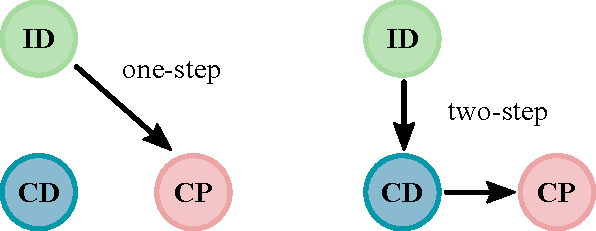
\includegraphics[width=0.5\textwidth]{fig4a} \\ [40pt] 
        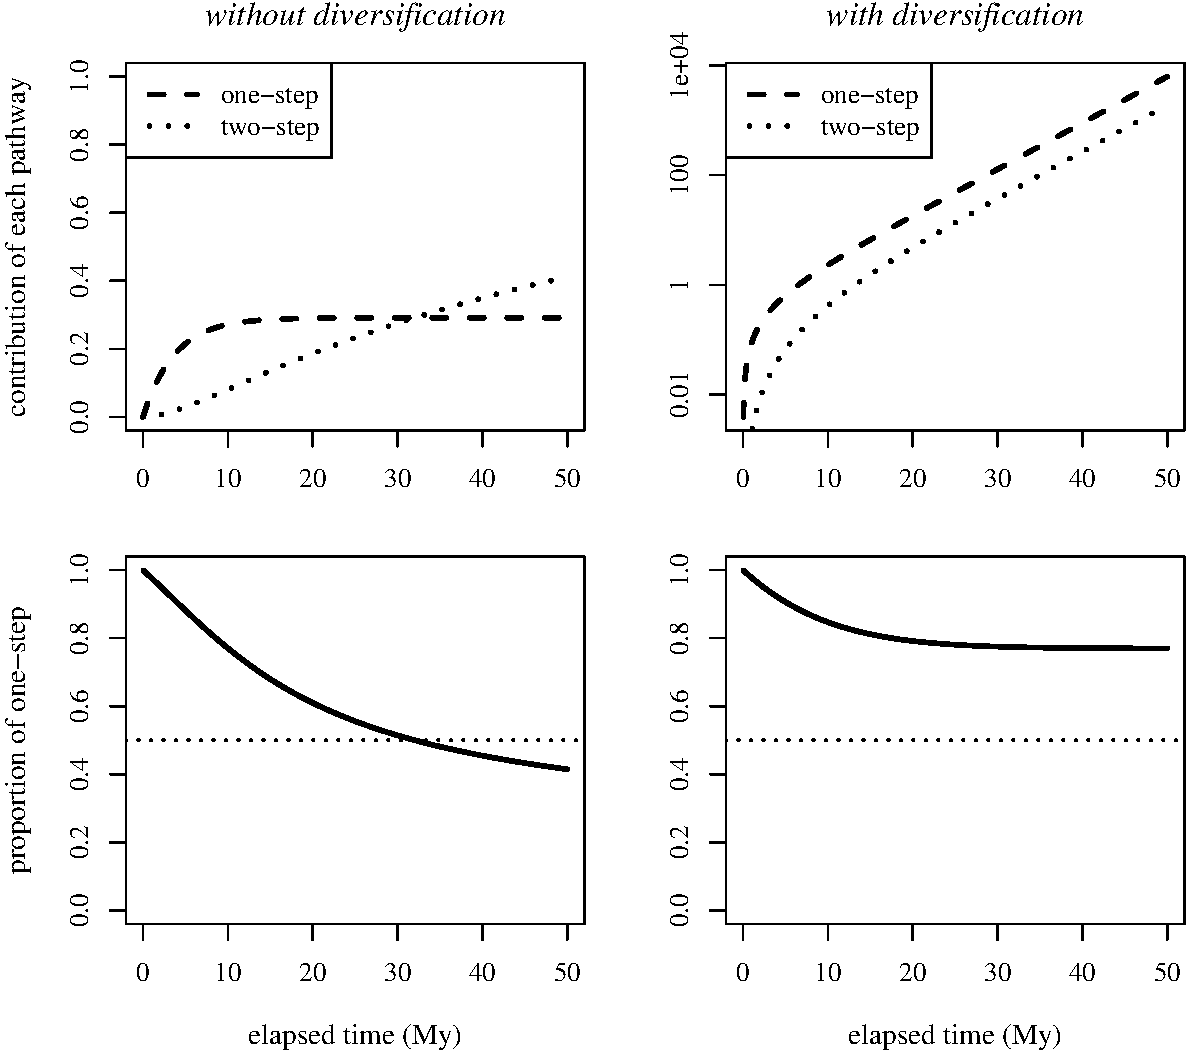
\includegraphics[width=0.9\textwidth]{fig4b}
    \caption{
        Contributions of the two pathways to polyploidy.
        The one-step pathway is direct ID$\rightarrow$CP transitions.
        The two-step pathway consists of ID$\rightarrow$CD$\rightarrow$CP transitions.
        When considering only rates of transitions among the states (ignoring the diversification rate parameters), the one-step pathway dominates on short timescales and the two-step on long timescales (left panels).
        When also considering diversification within each state, the one-step pathway, in which polyploidization breaks down SI, dominates over any timescale (right panels).
        The top panels show the separate contributions of each pathway.
        The bottom panels show the proportional contribution of the one-step pathway (\ie one-step / [one-step + two-step]).
    }
    \label{figure:pathways}
\end{figure}


% check values of delta and rho D/P+A/B with(out) delta
% i.e. parameter values in figure S1 & S4 vs Table S2
\begin{suppfigure}
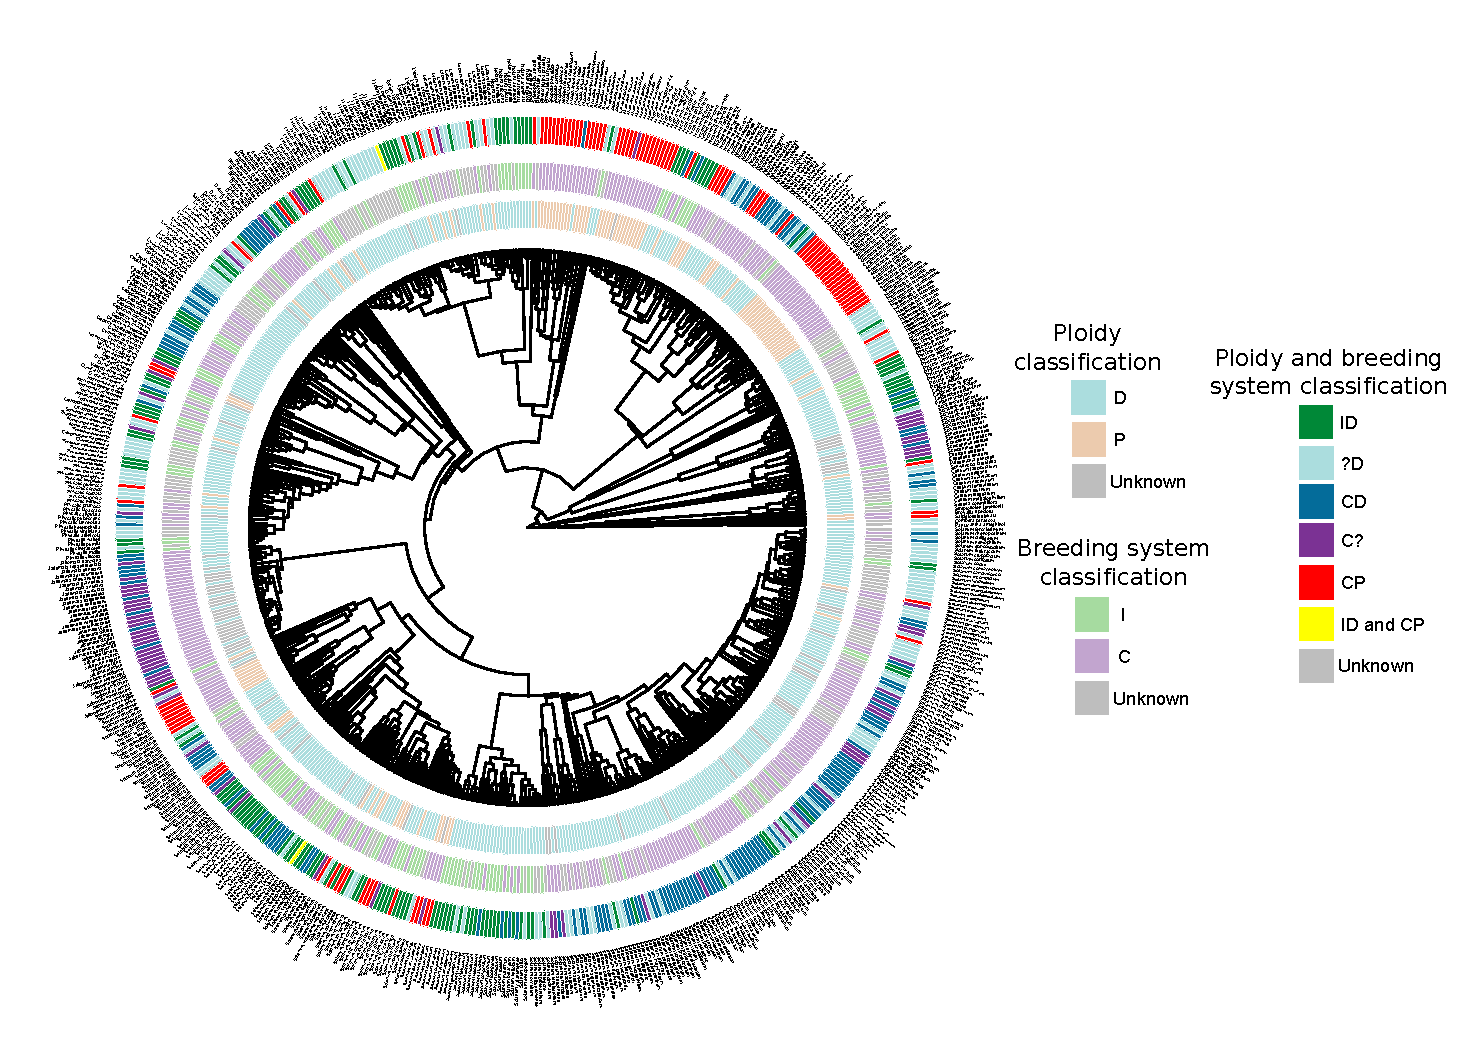
\includegraphics[width=\textwidth]{figS1.pdf}
    \caption{Ploidy and breeding system data according to three different classifications. For ploidy only models, classifications with states $D$ and $P$ were used (inner circle). For breeding system models classifications with states $I$ and $C$ were used (middle circle). For ploidy and breeding system models classifications using $ID, CD, CP$ were used (outer circle). Data with missing information in one of the traits was classified simultaneously as two possible states, for example, diploids without breeding system $?D$ were classified as $(CD, CP)$).}
    \label{fig:allmodels}
\end{suppfigure}



\begin{suppfigure}% figS2 models
    \caption{ Twenty-nine models of diversification are proposed for the study of ploidy, breeding systems, and hidden states linked to the process of diversification. We divide the models by the type of focal trait studied (ploidy only, breeding system only, or ploidy and breeding system). The contributions of the focal trait to the diversification process can be measured by comparing the models in each of the columns. That is, the focal trait only models assume that speciation and extinction rates are only linked to the trait itself, the hidden trait only models assume that the diversification rates are  linked to unknown factors but not the trait of interest, and the focal trait with hidden trait models assume that both the focal trait and unknown factors are contributing to diversification.}
    \label{fig:allmodels}
\end{suppfigure}



\begin{suppfigure}
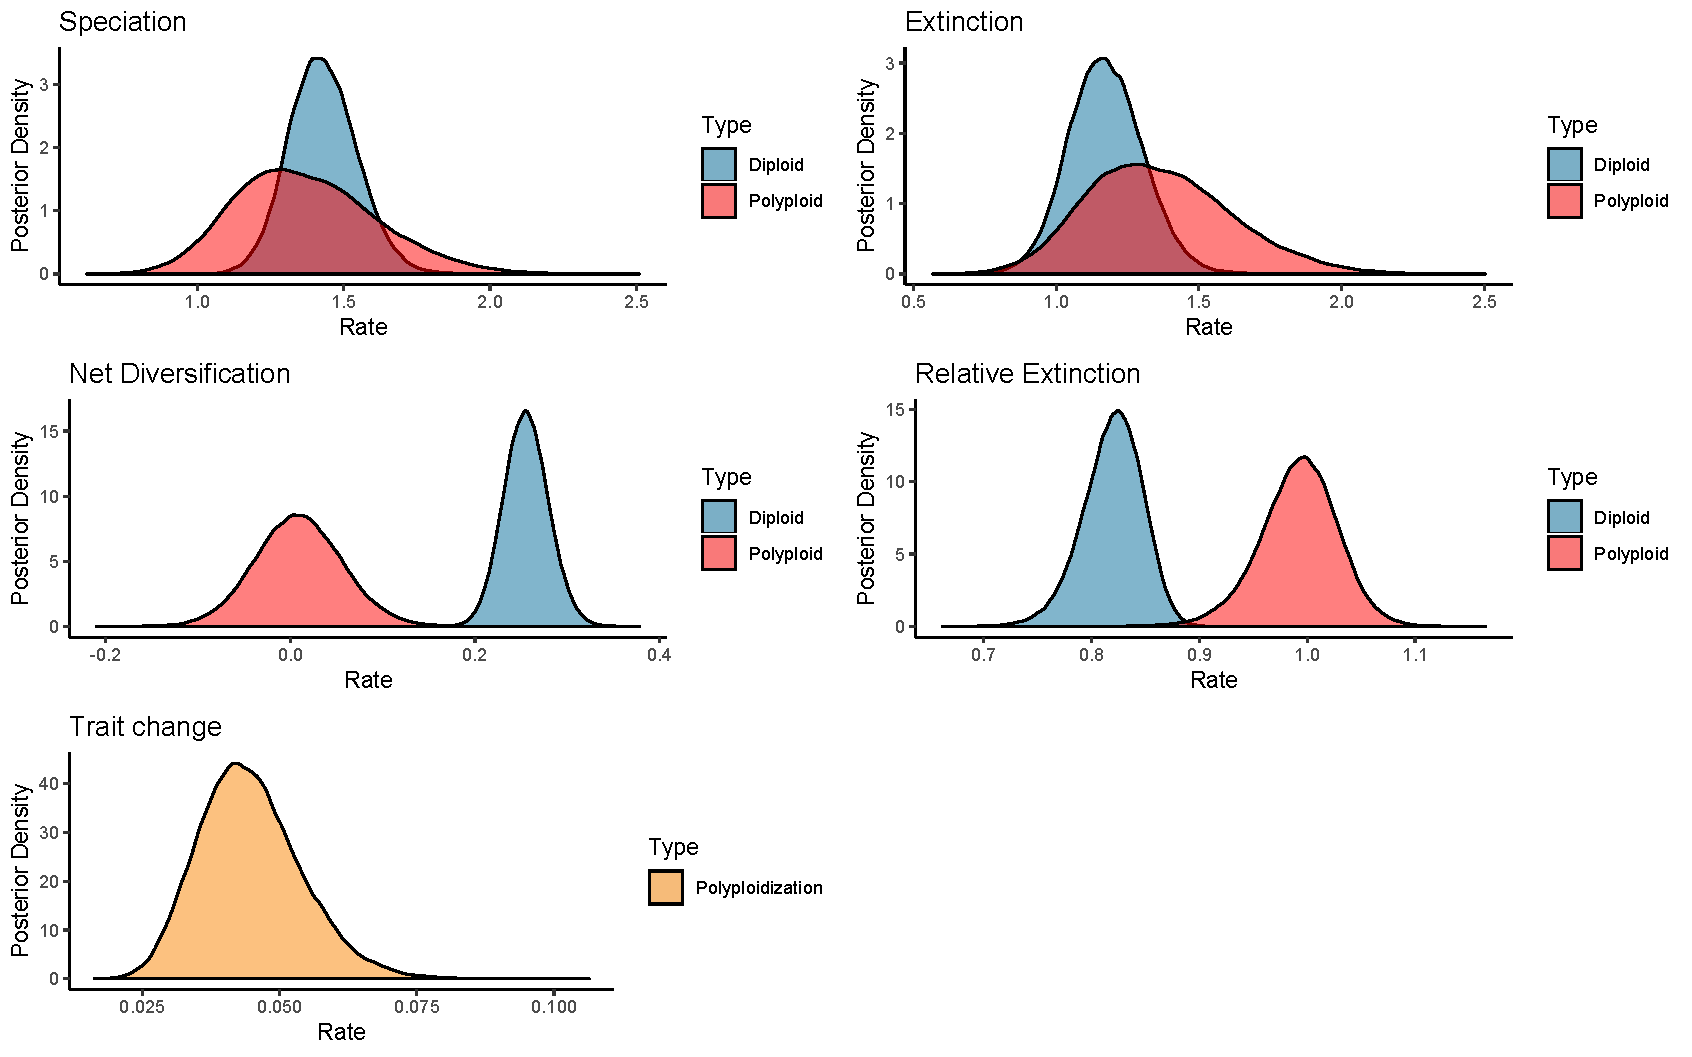
\includegraphics[width=\textwidth]{figS3.pdf}
\caption{Posterior distributions for each of the parameters in the ploidy only model (M1). Red color represents diploid state $D$ and blue color represents polyploid state $P$.  (A)Speciation rates. (B) Extinction rates. (C) Net diversification rates (speciation minus extinction from panels A and B). (D) Relative extinction rates (extinction divided by speciation from panels A and B). (E) Polyploidization rate ($\rho$).} % XXX
\label{suppfigure:DPnodip}
\end{suppfigure}

\begin{suppfigure}
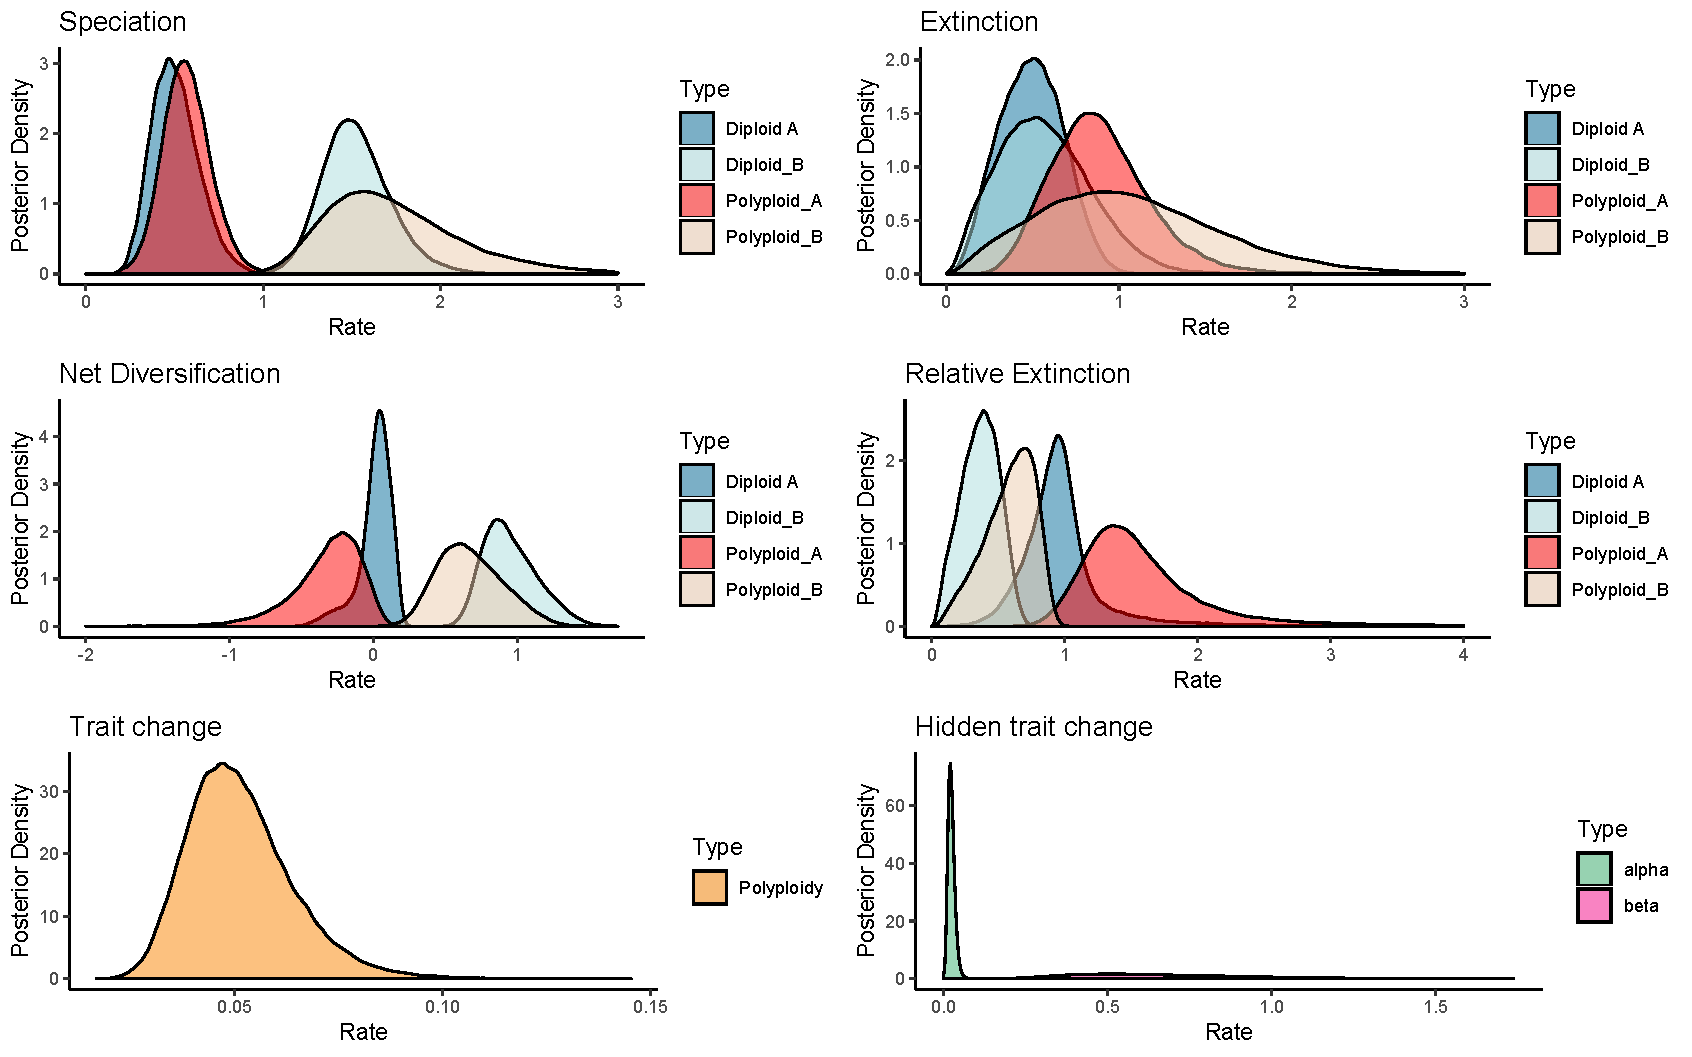
\includegraphics[width=\textwidth]{figS4.pdf}
\caption{Posterior distributions for each of the parameters in the ploidy and hidden trait model (M4). Red color represents diploid state $D$ and blue color represents polyploid state $P$. Dark colors represent hidden state $A$ and light colors hidden state $B$.  (A) Speciation rates. (B) Extinction rates. (C) Net diversification rates (speciation minus extinction from panels A and B). (D) Relative extinction rates (extinction divided by speciation from panels A and B). (E) Polyploidization rate ($\rho$). (F) Transition rates between hidden states ( $\alpha$ and $\beta$).} % XXX
\label{suppfigure:DPnodipAB}
\end{suppfigure}

\begin{suppfigure}
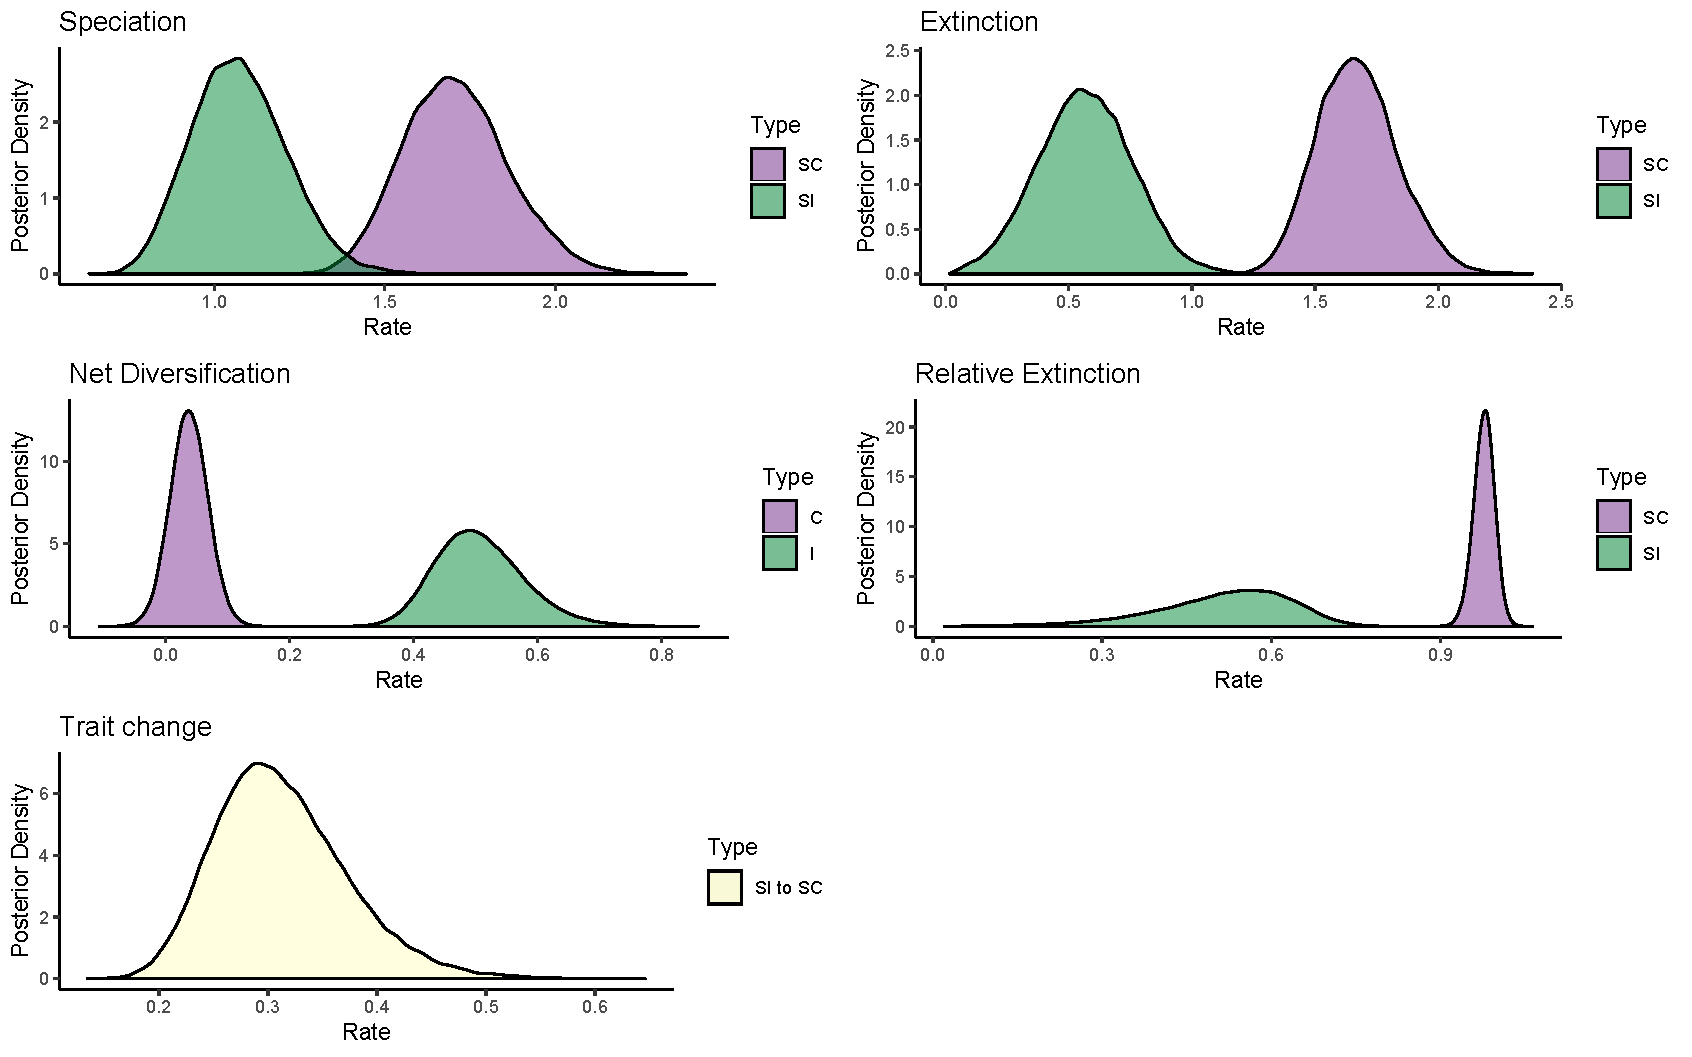
\includegraphics[width=\textwidth]{figS5.pdf}
\caption{Posterior distributions for each of the parameters in the breeding system only model (M11). Green color represents self-incompatible state $I$ and purple color represents self-compatible state $C$.  (A) Speciation rates. (B) Extinction rates. (C) Net diversification rates (speciation minus extinction from panels A and B). (D) Relative extinction rates (extinction divided by speciation from panels A and B). (E) Self-incompatible to self-compatible transition rate ($q_IC$).} % XXX
\label{suppfigure:IC}
\end{suppfigure}


\begin{suppfigure}
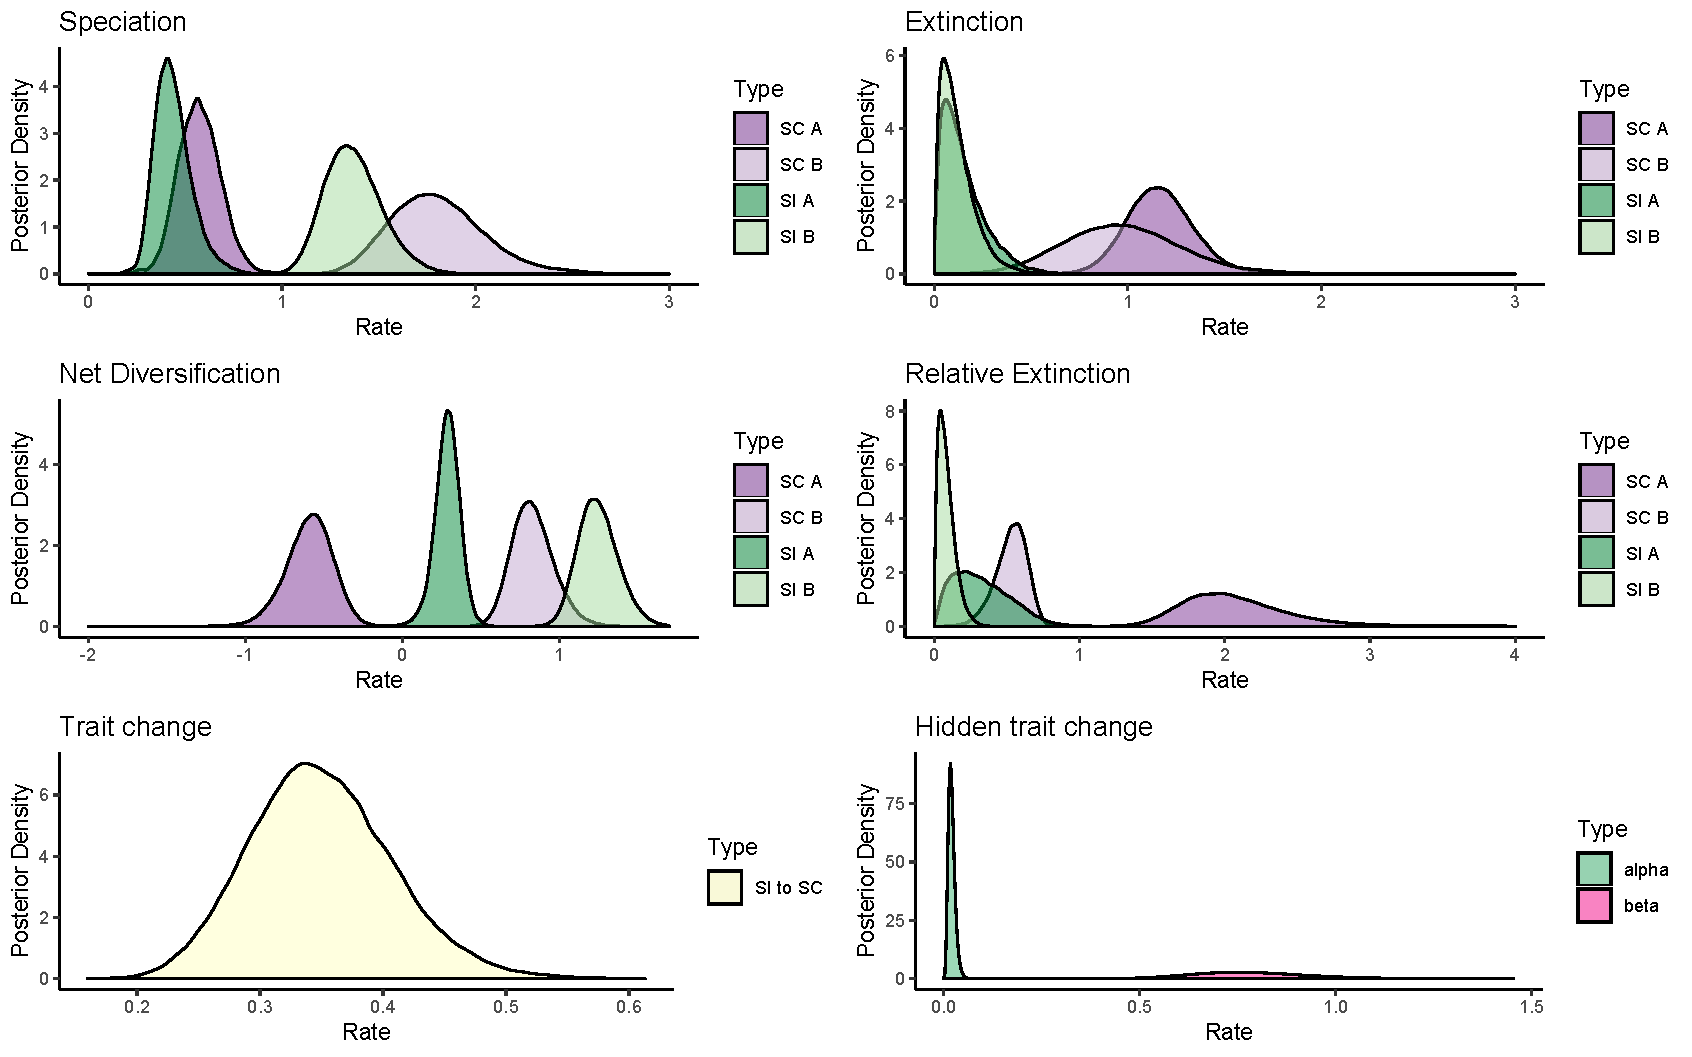
\includegraphics[width=\textwidth]{figS6.pdf}
\caption{Posterior distributions for each of the parameters in the breeding system and hidden trait model (M14). Green color represents self-incompatible state $I$ and purple color represents self-compatible state $A$. Dark colors represent hidden state $A$ and light colors hidden state $B$.  (A) Speciation rates. (B) Extinction rates. (C) Net diversification rates (speciation minus extinction from panels A and B). (D) Relative extinction rates (extinction divided by speciation from panels A and B). (E) Self-incompatible to self-compatible transition rate ($q_IC$). (F) Transition rates between hidden states ( $\alpha$ and $\beta$).} % XXX
\label{suppfigure:ICAB}
\end{suppfigure}


\begin{suppfigure}
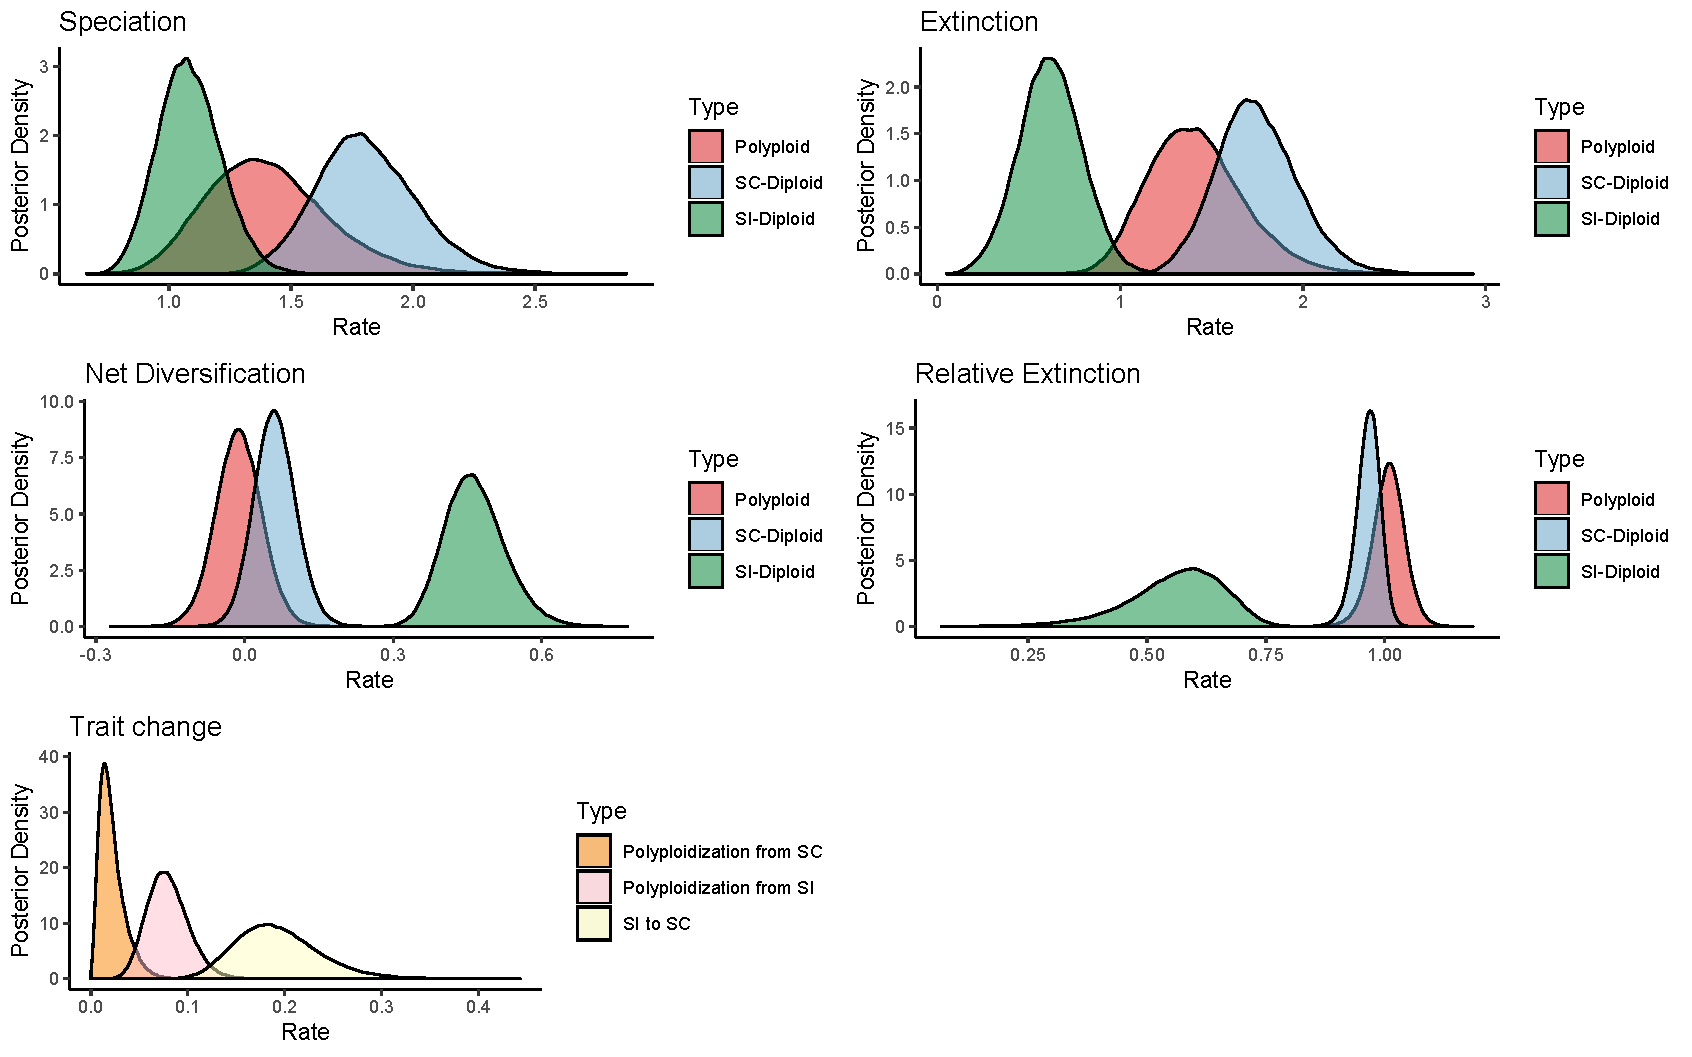
\includegraphics[width=\textwidth]{figS7.pdf}
\caption{Posterior distribution for each of the parameters in the ploidy and breeding system model (M16). Green color represents self-incompatible diploid state $ID$, blue color is the self-compatible and diploid state $CD$ and pink represents self-compatible polyploid state $CP$.  (A) Speciation rates. (B) Extinction rates. (C) Net diversification rates (speciation minus extinction from panels A and B). (D) Relative extinction rates (extinction divided by speciation from panels A and B). (E) Self-incompatible to self-compatible transition rate ($q_IC$, yellow), polyploidization rate from self-incompatible ($\rho_I,$ light pink), and polyploidization from self-compatible ($\rho_c$, orange).} % XXX
\label{suppfigure:IDCDCPnodip}
\end{suppfigure}

\begin{suppfigure}
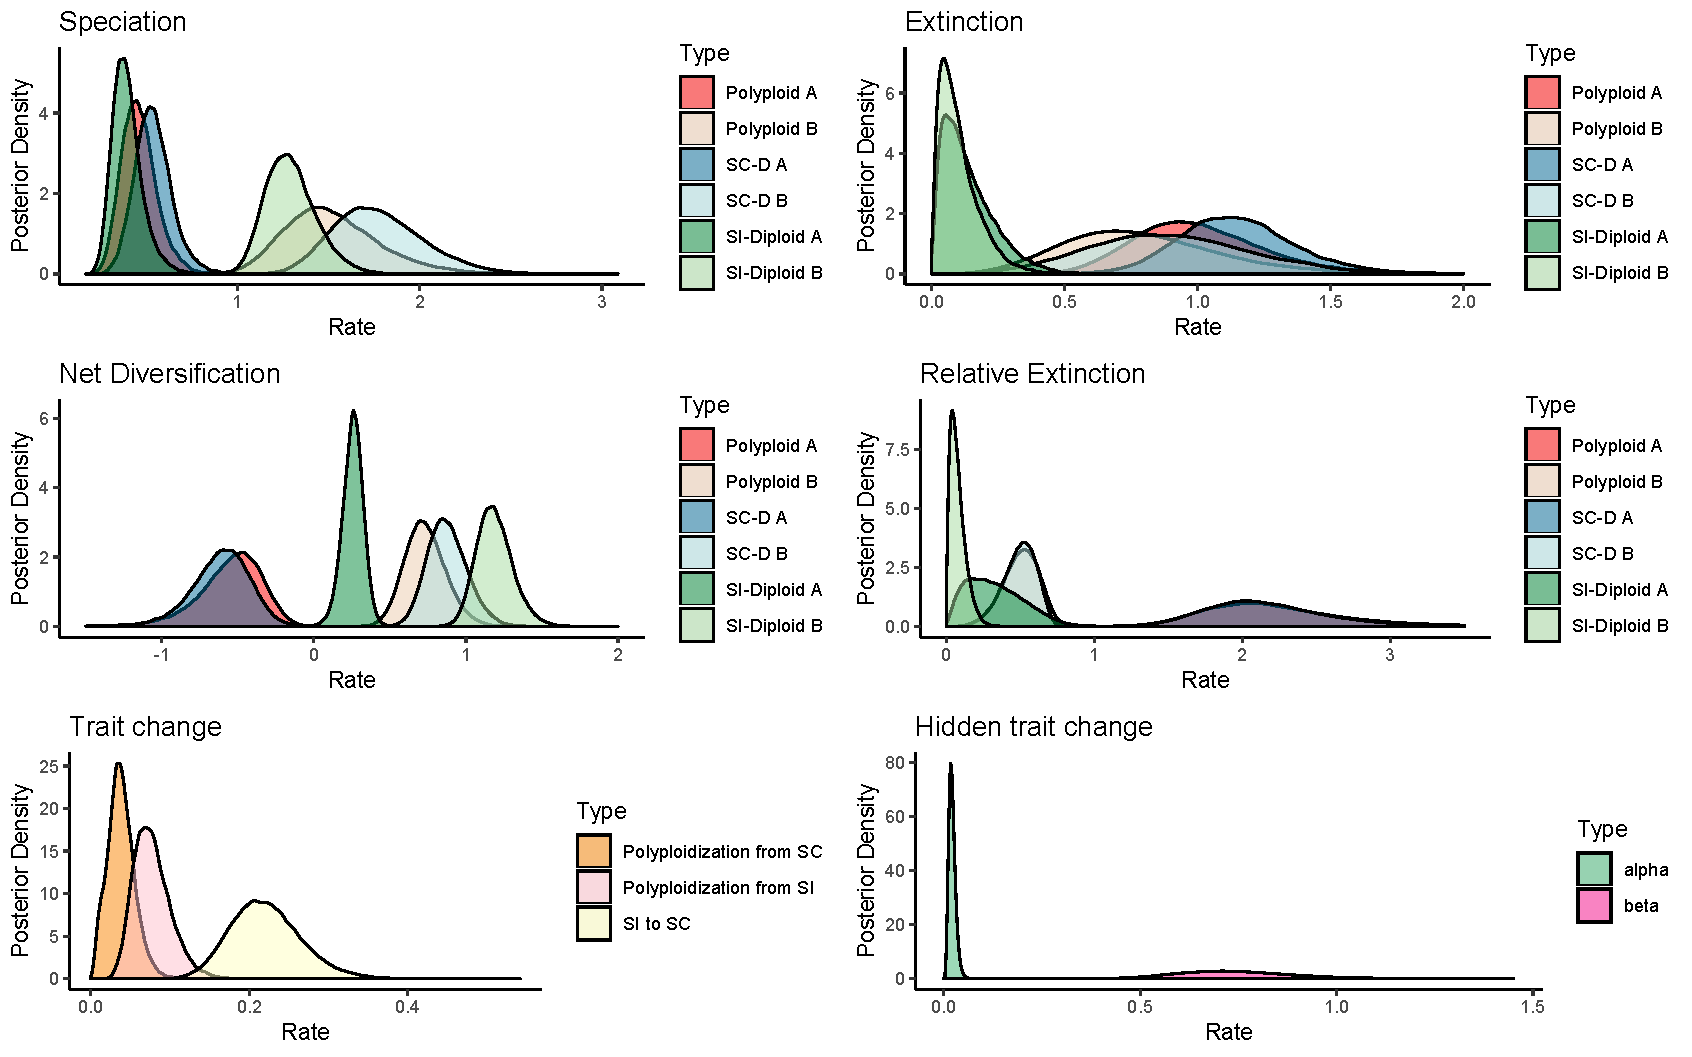
\includegraphics[width=\textwidth]{figS8.pdf}
\caption{Posterior distribution for each of the parameters in the ploidy, breeding system, and hidden trait model (M19). Green color represents self-incompatible diploid state $ID$, blue color is the self-compatible and diploid state $CD$ and pink represents self-compatible polyploid state $CP$. Dark colors represent hidden state $A$ and light colors hidden state $B$.  (A) Speciation rates. (B) Extinction rates. (C) Net diversification rates (speciation minus extinction from panels A and B). (D) Relative extinction rates (extinction divided by speciation from panels A and B). (E) Self-incompatible to self-compatible transition rate ($q_IC$, yellow), polyploidization rate from self-incompatible ($\rho_I,$ light pink), and polyploidization from self-compatible ($\rho_c$, orange). (F) Transition rates between hidden states ( $\alpha$ and $\beta$).}% XXX
\label{suppfigure:IDCDCPnodipAB}
\end{suppfigure}

\begin{suppfigure}
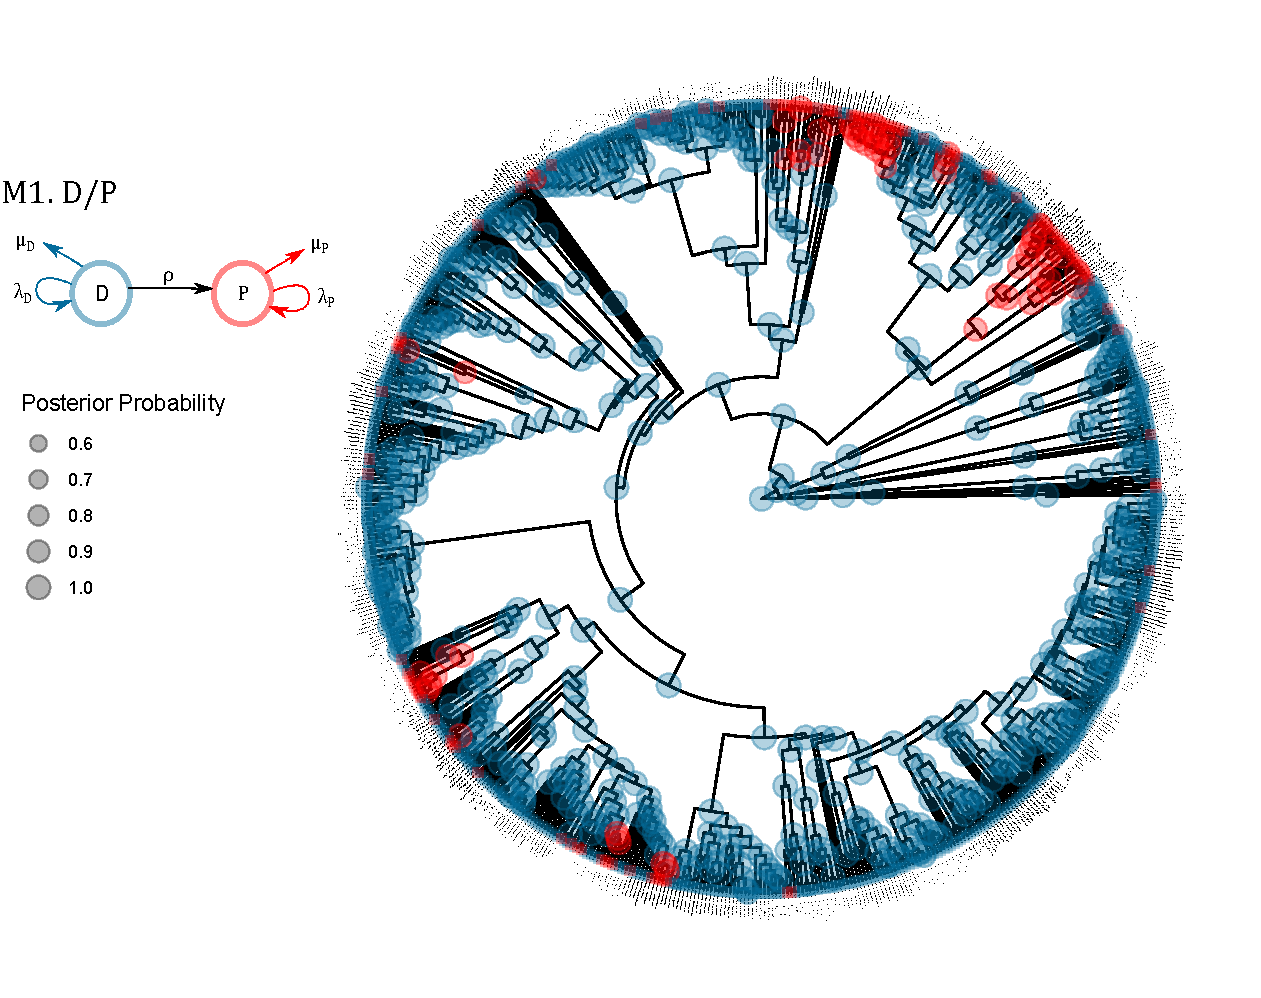
\includegraphics[width=\textwidth]{figS9.pdf}
\caption{Ancestral state estimation showing the maximum \emph{a posteriori} estimates of the marginal probability distributions for each of the 650 internal nodes under  the ploidy only model (M1). } % XXX
\label{suppfigure:DPnodipasr}
\end{suppfigure}



\begin{suppfigure}
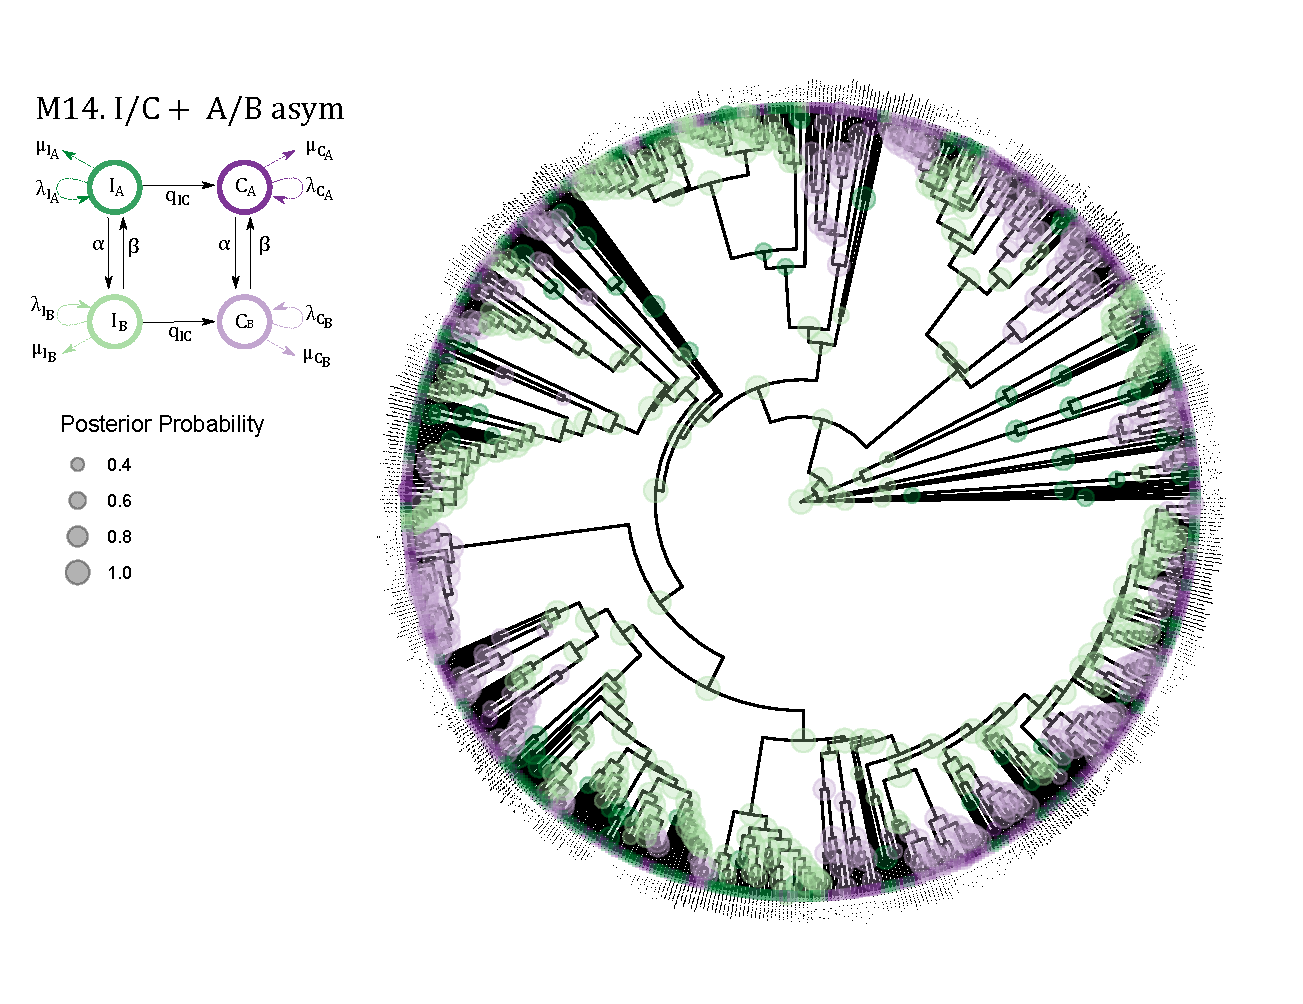
\includegraphics[width=\textwidth]{figS12.pdf}
\caption{Ancestral state estimation showing the maximum \emph{a posteriori} estimates of the marginal probability distributions for each of the 650 internal nodes under the ploidy and hidden states model (M4).} % XXX
\label{suppfigure:DPnodipABasr}
\end{suppfigure}


\begin{suppfigure}
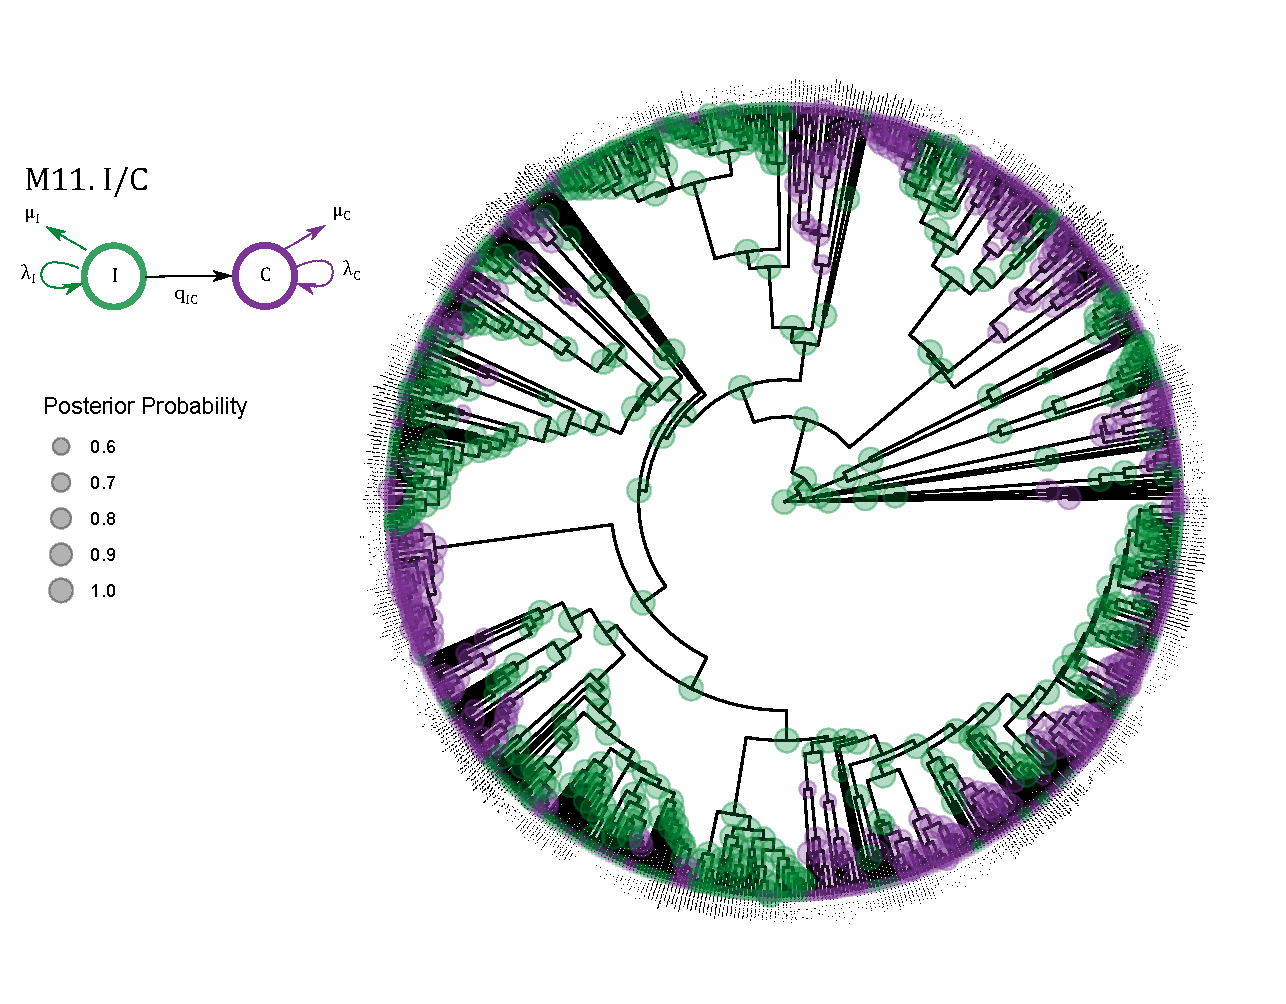
\includegraphics[width=\textwidth]{figS11.pdf}
\caption{Ancestral state estimation showing the maximum \emph{a posteriori} estimates of the marginal probability distributions for each of the 650 internal nodes under the  breeding system only model (M11).} % XXX
\label{suppfigure:ICasr}
\end{suppfigure}



\begin{suppfigure}
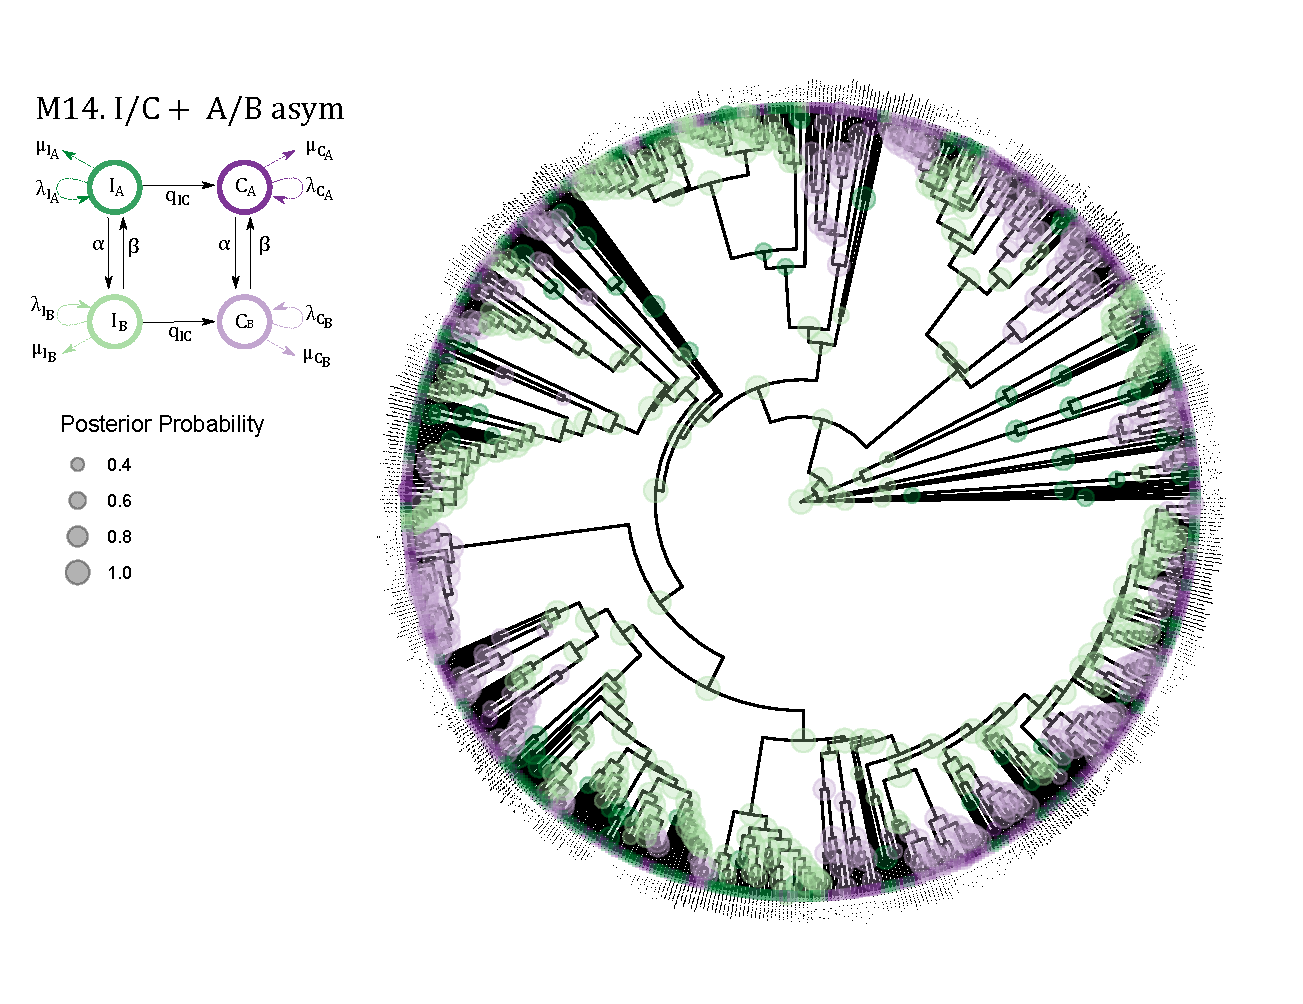
\includegraphics[width=\textwidth]{figS12.pdf}
\caption{Ancestral state estimation showing the maximum \emph{a posteriori} estimates of the marginal probability distributions for each of the 650 internal nodes under the breeding system and hidden states model (M14.} % XXX
\label{suppfigure:ICABasr}
\end{suppfigure}


\begin{suppfigure}
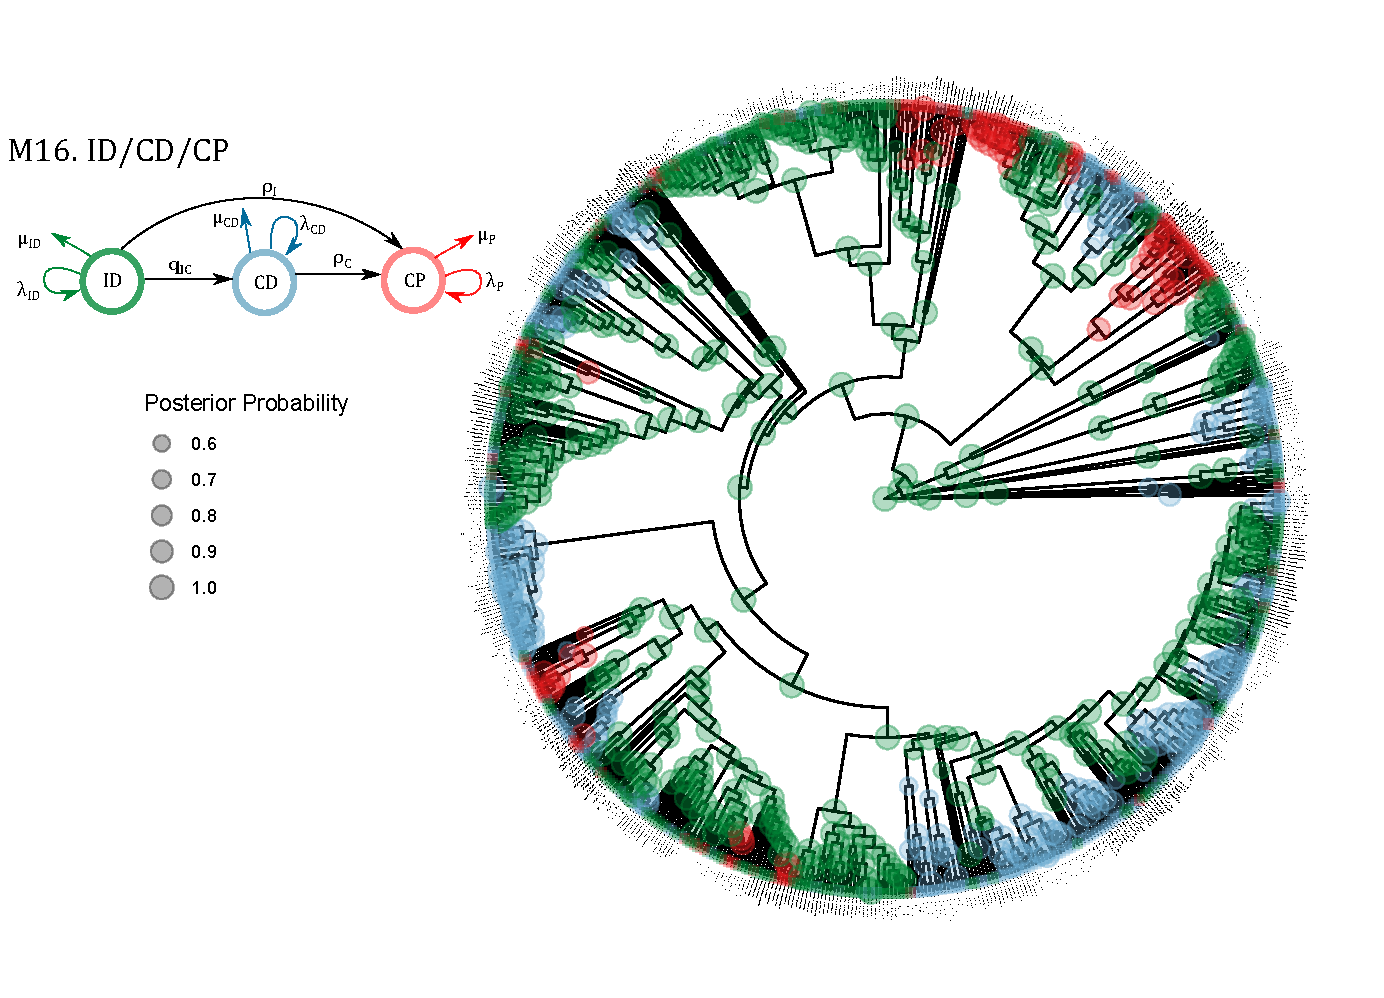
\includegraphics[width=\textwidth]{figS13.pdf}
\caption{Ancestral state estimation showing the maximum \emph{a posteriori} estimates of the marginal probability distributions for each of the 650 internal nodes under the ploidy and breeding system model (M16).} % XXX
\label{suppfigure:IDCDCPnodipasr}
\end{suppfigure}



\begin{suppfigure}
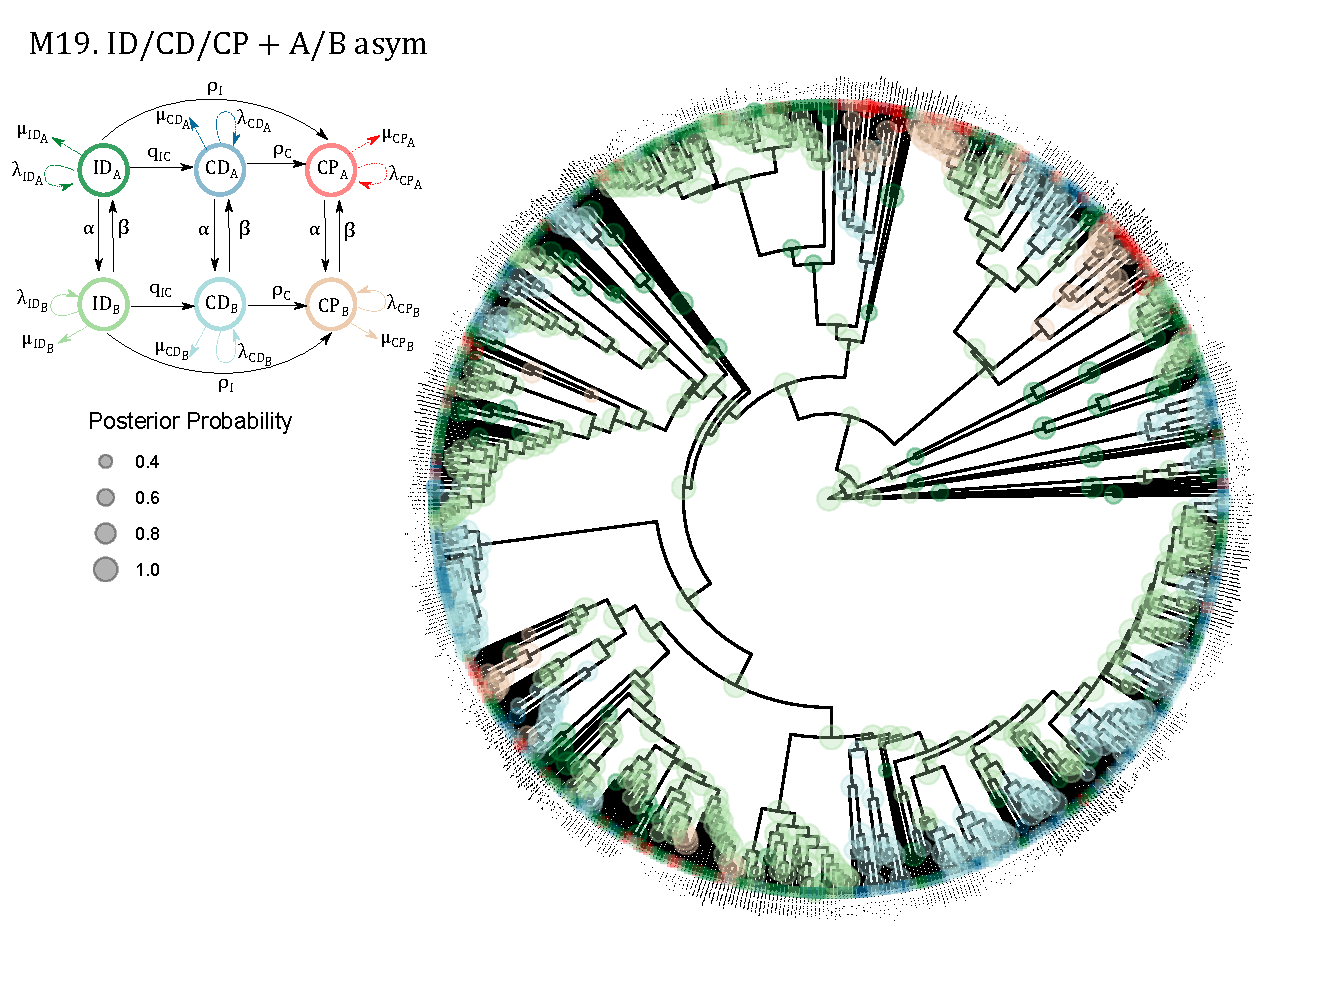
\includegraphics[width=\textwidth]{figS14.pdf}
\caption{Ancestral state estimation showing the maximum \emph{a posteriori} estimates of the marginal probability distributions for each of the 650 internal nodes under the  ploidy, breeding systems, and hidden states model (M19).} % XXX
\label{suppfigure:IDCDCPnodipABasr}
\end{suppfigure}



\begin{suppfigure}
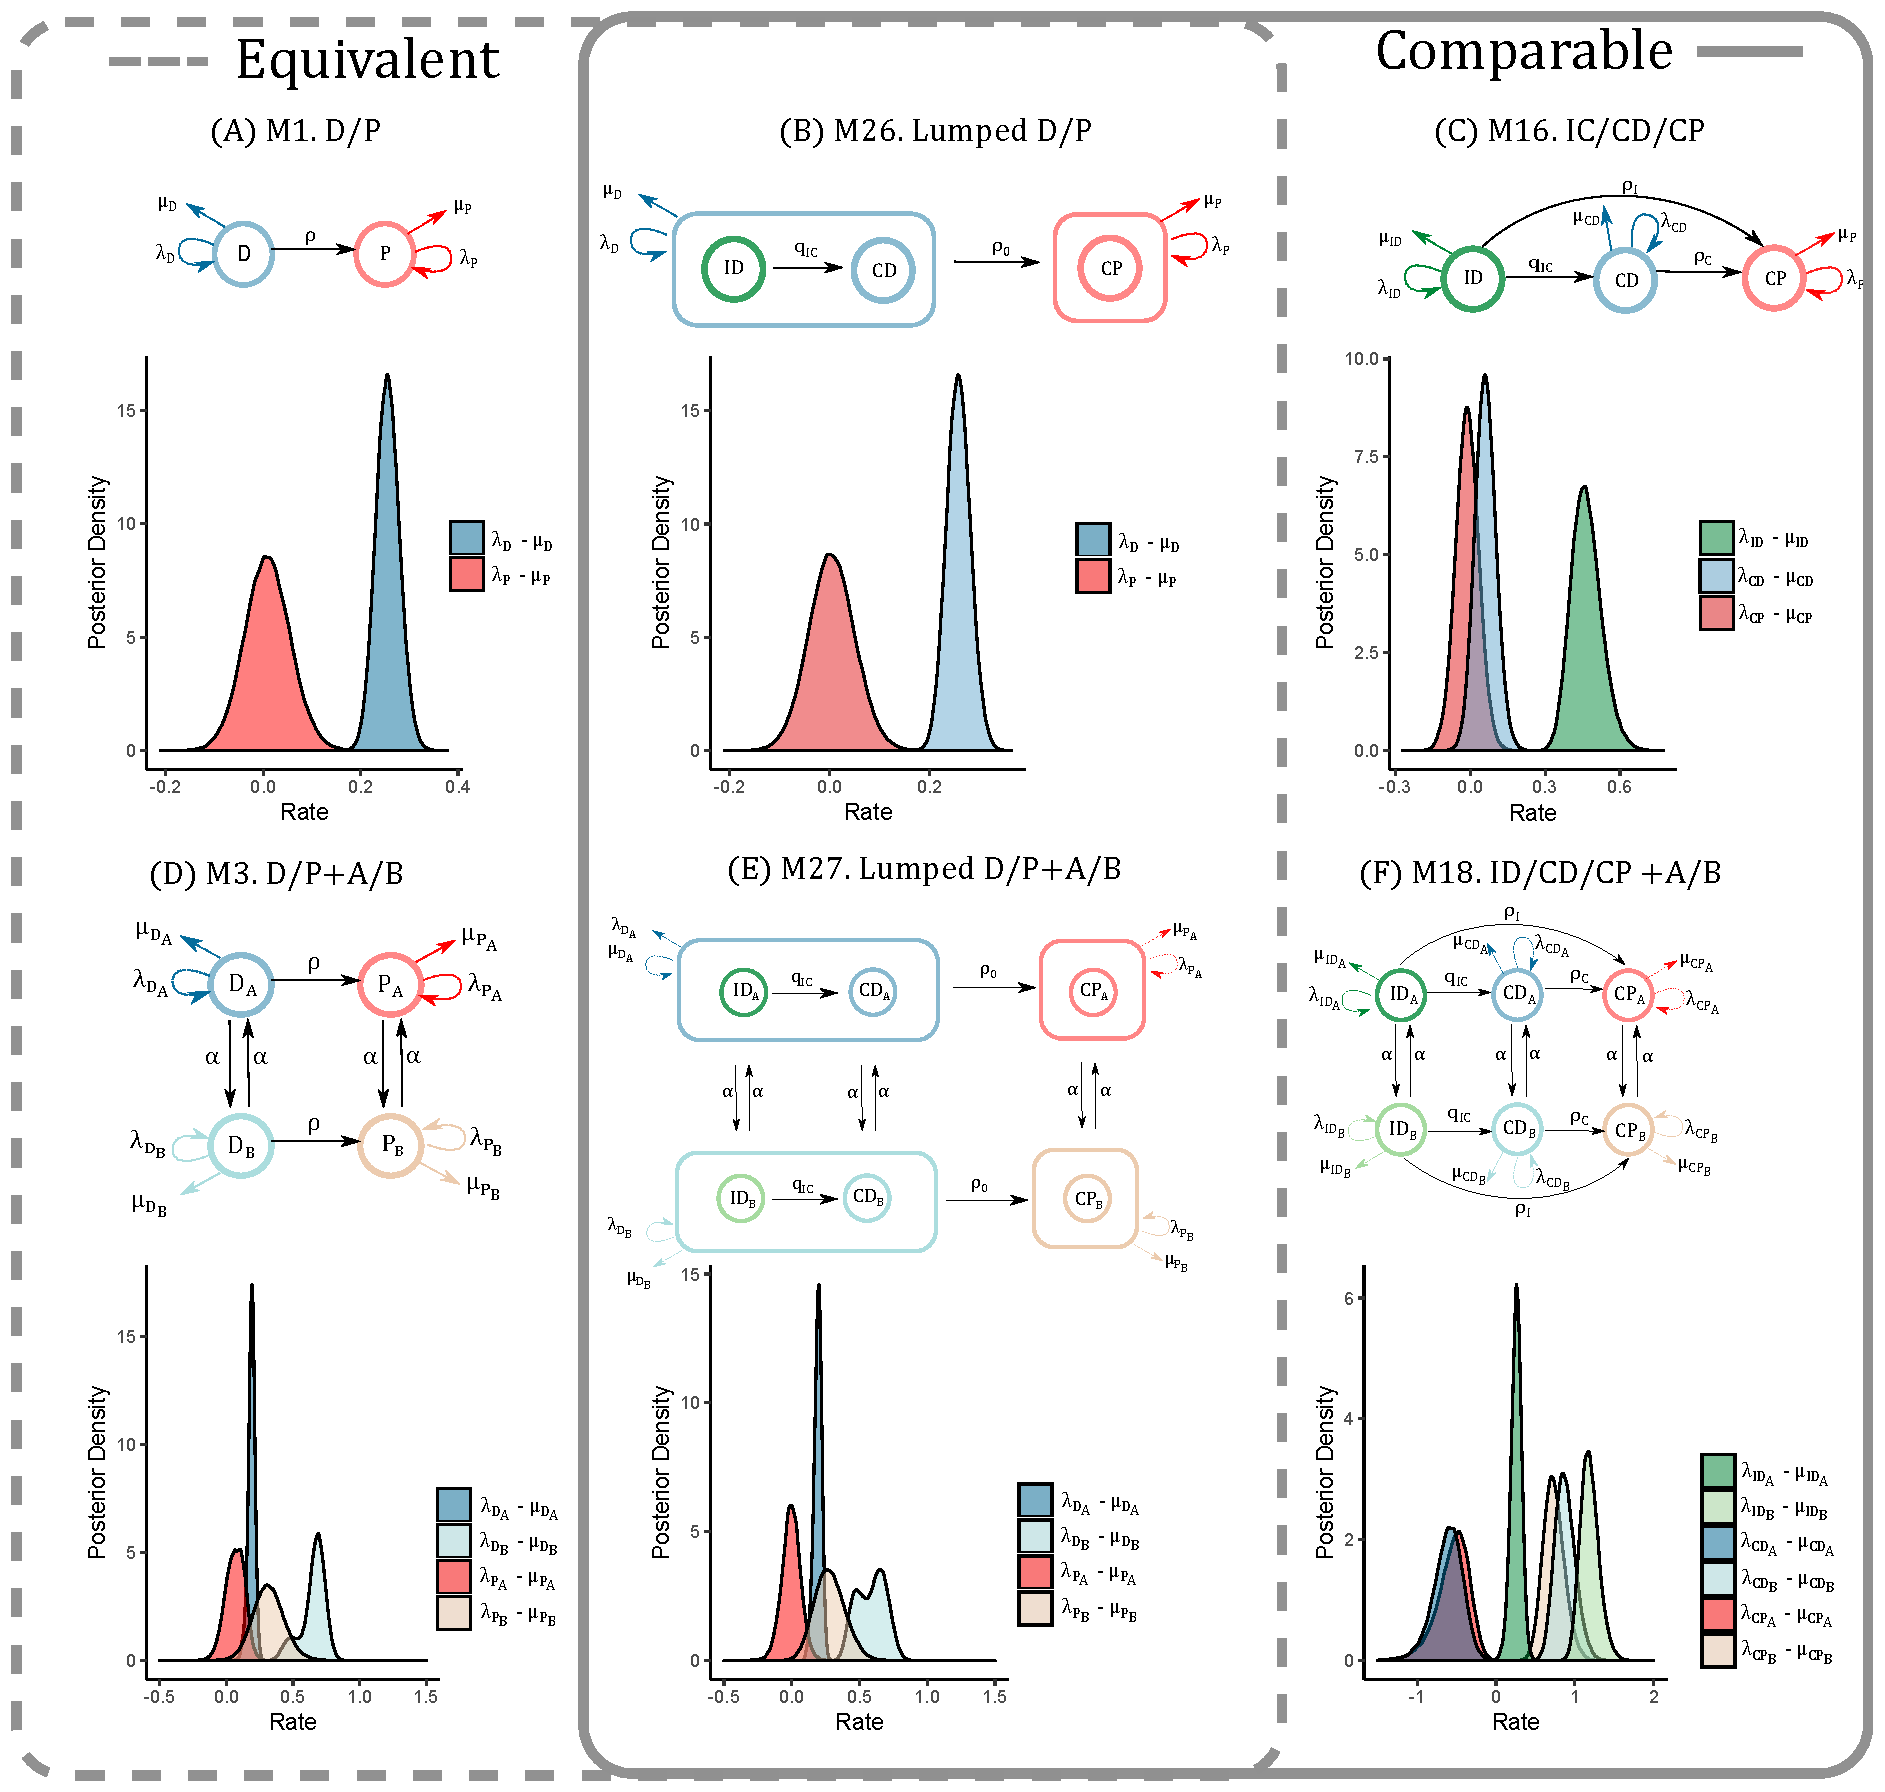
\includegraphics[width=\textwidth]{figS15.pdf}
\caption{Testing the addition of breeding system to ploidy models. (A) Ploidy only model (M1) where data enter as binary $D$ and $P$. (B) Lumped model for ploidy (M26) where data are the three-state values ($ID,CP,CD$) but results are equivalent to model M1.  (C) Ploidy and breeding system model (M16) where  data enter as the three-state values. Models M26 and M16 are comparable whereas M1 and M16 are not. (D) Ploidy and hidden state model (M3) where data enter as binary $D$ and $P$. (E) Lumped model for ploidy and hidden state (M27) where data are the three-state values ($ID,CP,CD$) but results are equivalent to model M3. (F) Ploidy, breeding system, and hidden state model (M18) where  data enter as the three-state values. Models M27 and M18 are comparable whereas M3 and M18 are not. Bayes factors comparing the models are shown in \cref{table:lumped}.} % XXX
\label{suppfigure:lumpedDP}
\end{suppfigure}

\begin{suppfigure}
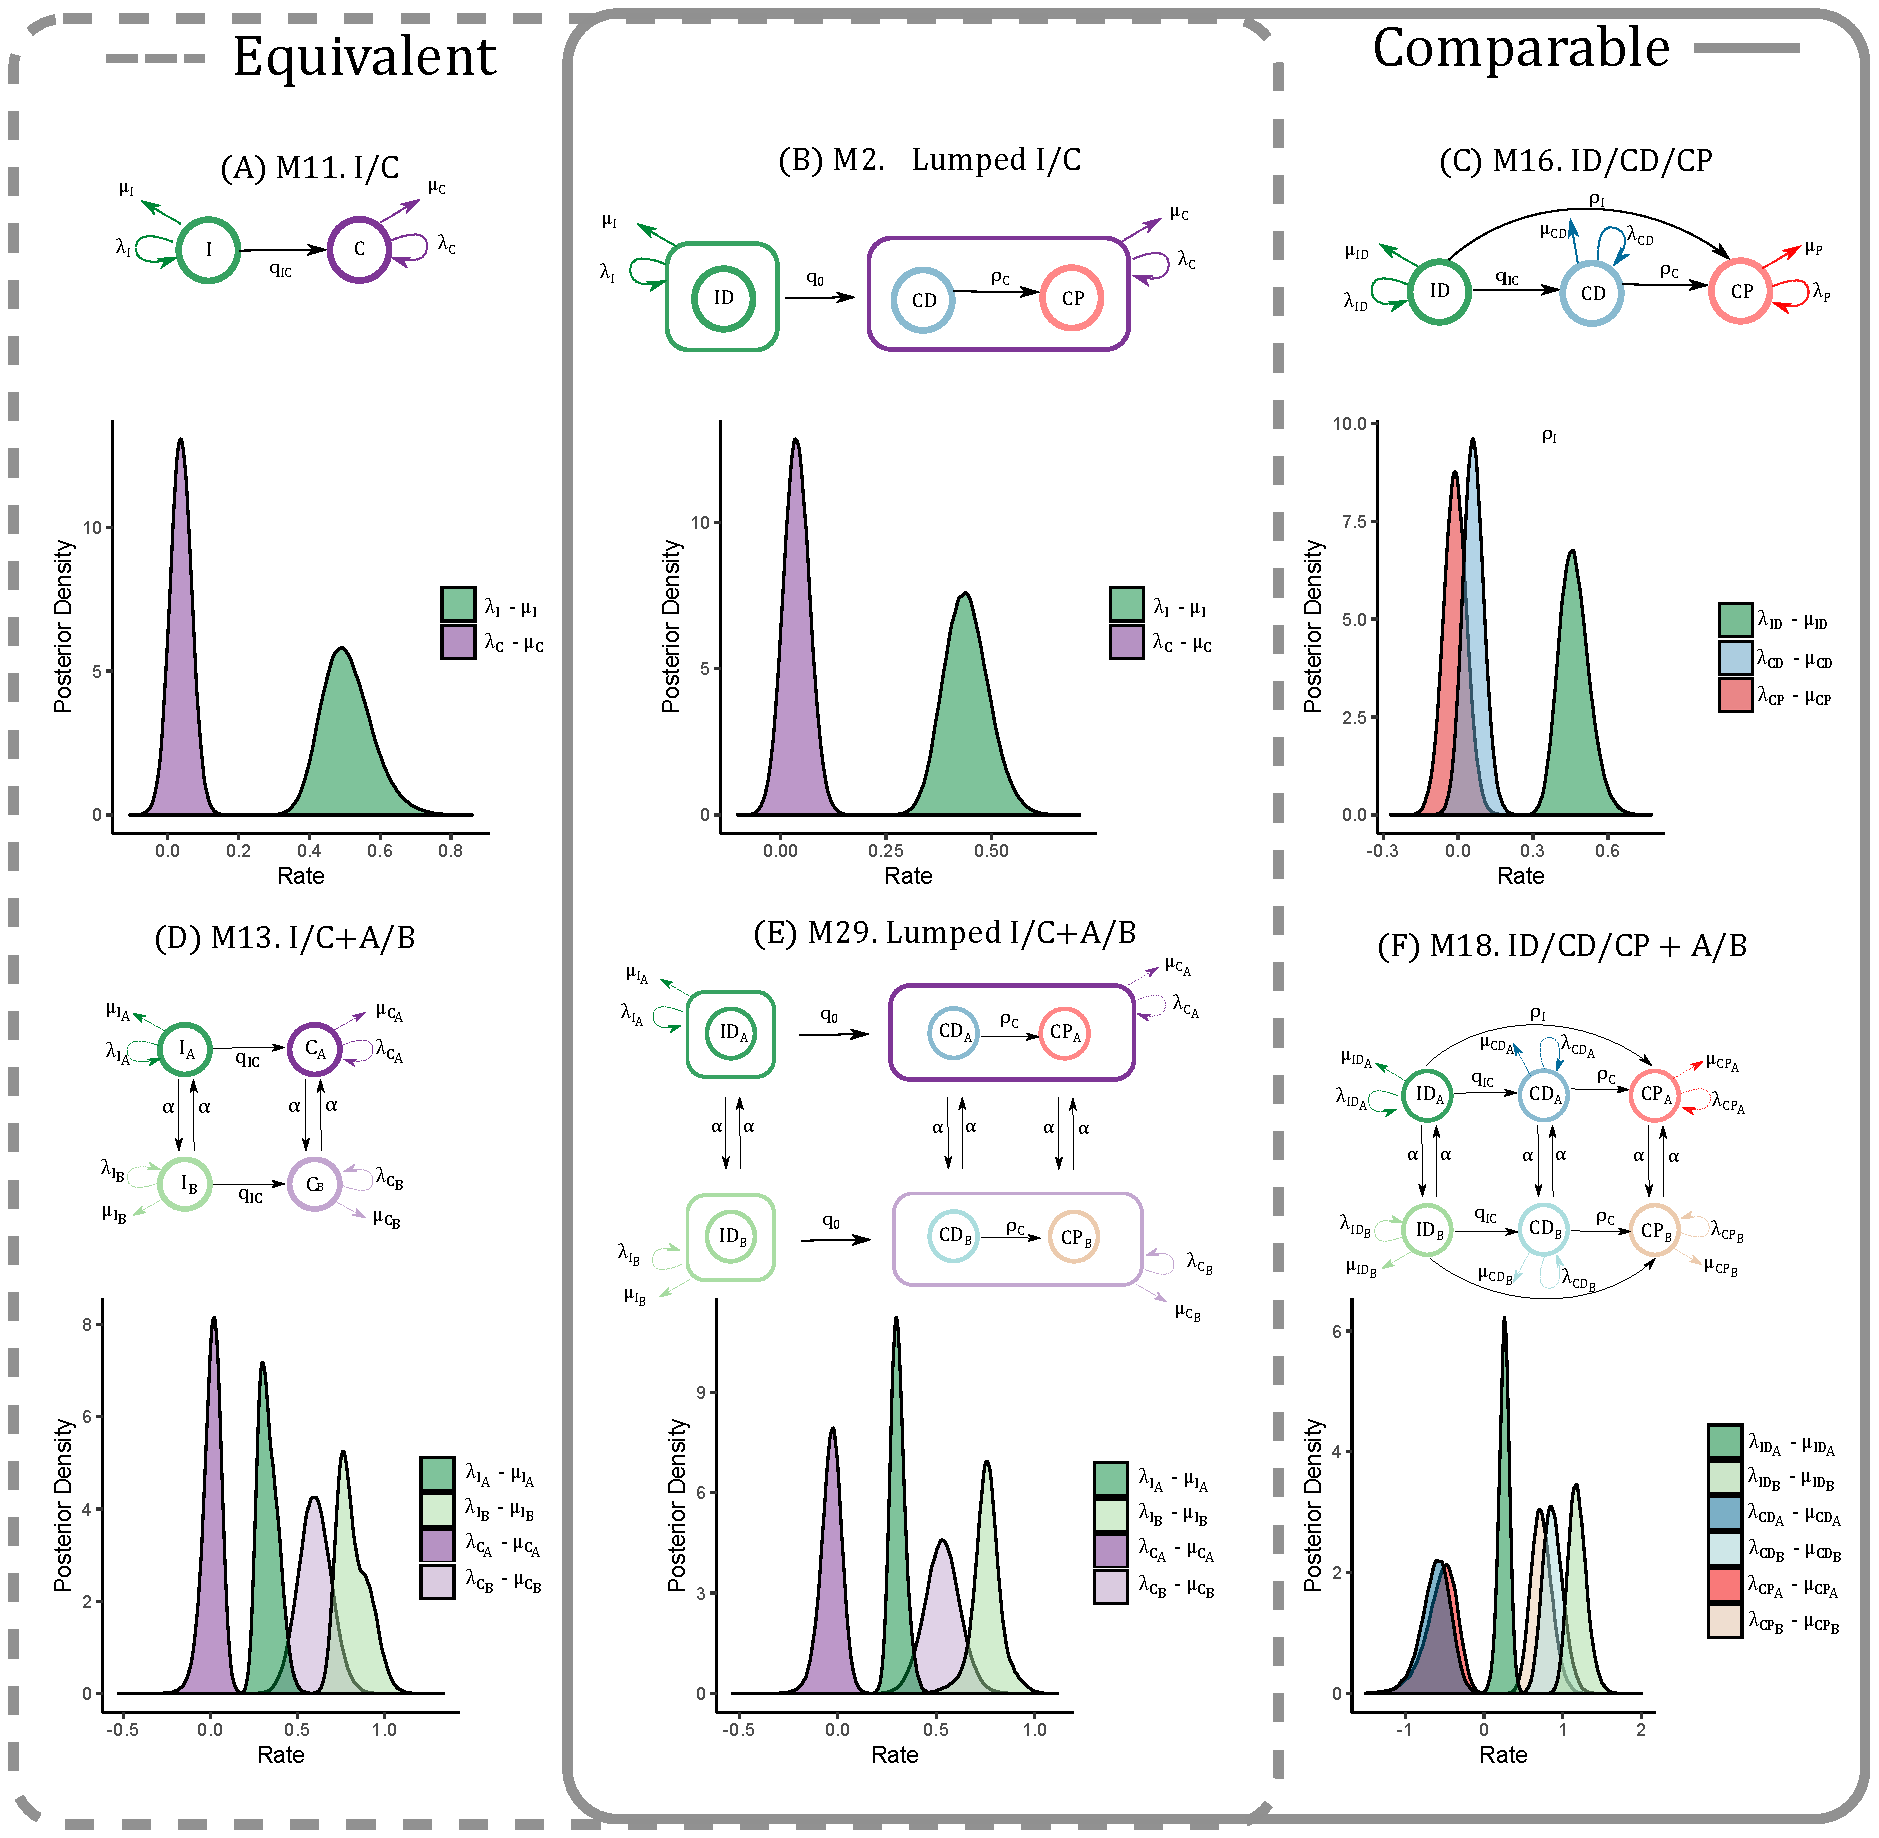
\includegraphics[width=\textwidth]{figS16.pdf}
\caption{Testing the addition of ploidy to breeding system models. (A) Breeding system only model (M11) where data enter as binary $I$ and $C$. (B) Lumped model for breeding system (M28) where data are the three-state values ($ID,CP,CD$) but results are equivalent to model M11.  (C) Ploidy and breeding system model (M16) where  data enter as the three-state values. Models M28 and M16 are comparable whereas M11 and M16 are not. (D) Breeding system and hidden state model (M13) where data enter as binary $I$ and $C$. (E) Lumped model for breeding system and hidden state (M29) where data are the three-state values ($ID,CP,CD$) but results are equivalent to model M13. (F) Ploidy, breeding system, and hidden state model (M18) where  data enter as the three-state values. Models M29 and M18 are comparable whereas M13 and M18 are not. Bayes factors comparing the models are shown in \cref{table:lumped}.} % XXX
\label{suppfigure:lumpedIC}
\end{suppfigure}


\begin{suppfigure}
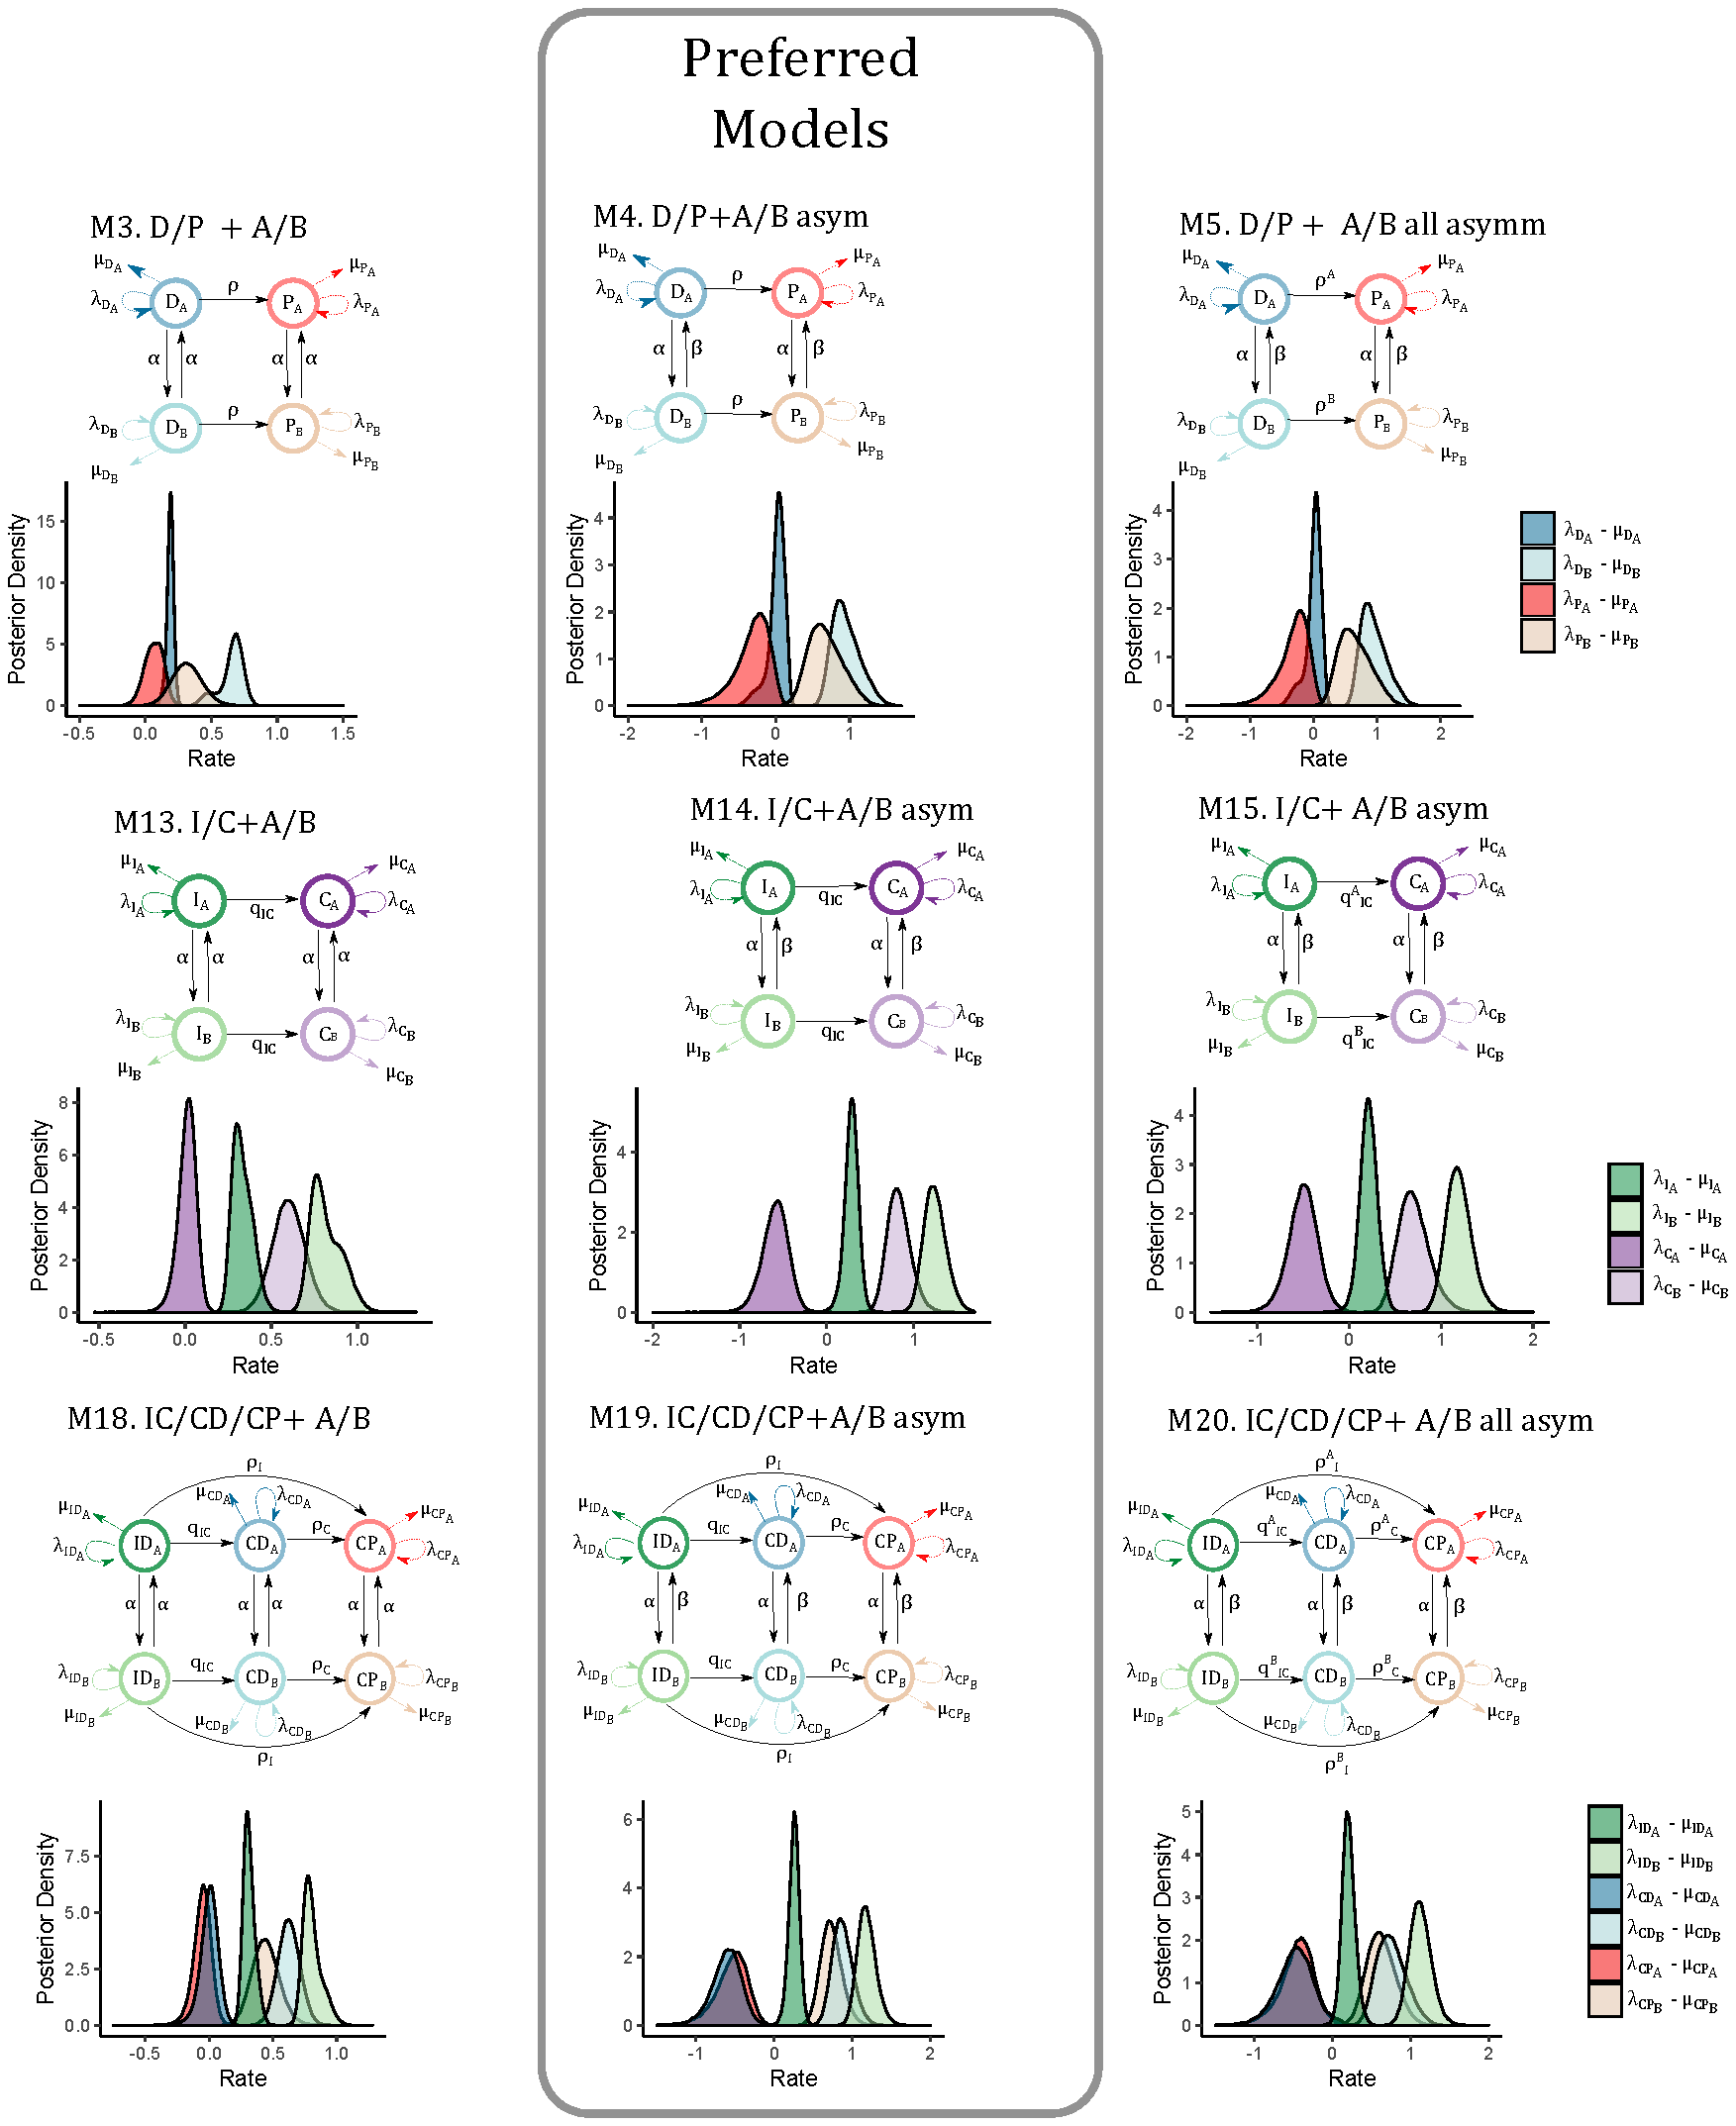
\includegraphics[width=\textwidth]{figS17.pdf}
\caption{Effect of asymmetric rates in hidden models. First column models M3, M13, and M18 assume that the rates between hidden states are equal. The models in the second column (M4, M14, M19) assume that the rates between hidden states are different . Column three models assumes that the rates between hidden state are asymmetric and that the transition rates within each hidden states are also different. Bayes factors in \cref{supptable:asymmetry} strongly preferred models with asymmetric rates between states (second column) over models with equal rates in hidden states (first column). Models in the second column are moderately or equally prefer to more complex models in column 3. } % XXX
\label{suppfigure:asymmetric}
\end{suppfigure}

\begin{suppfigure}
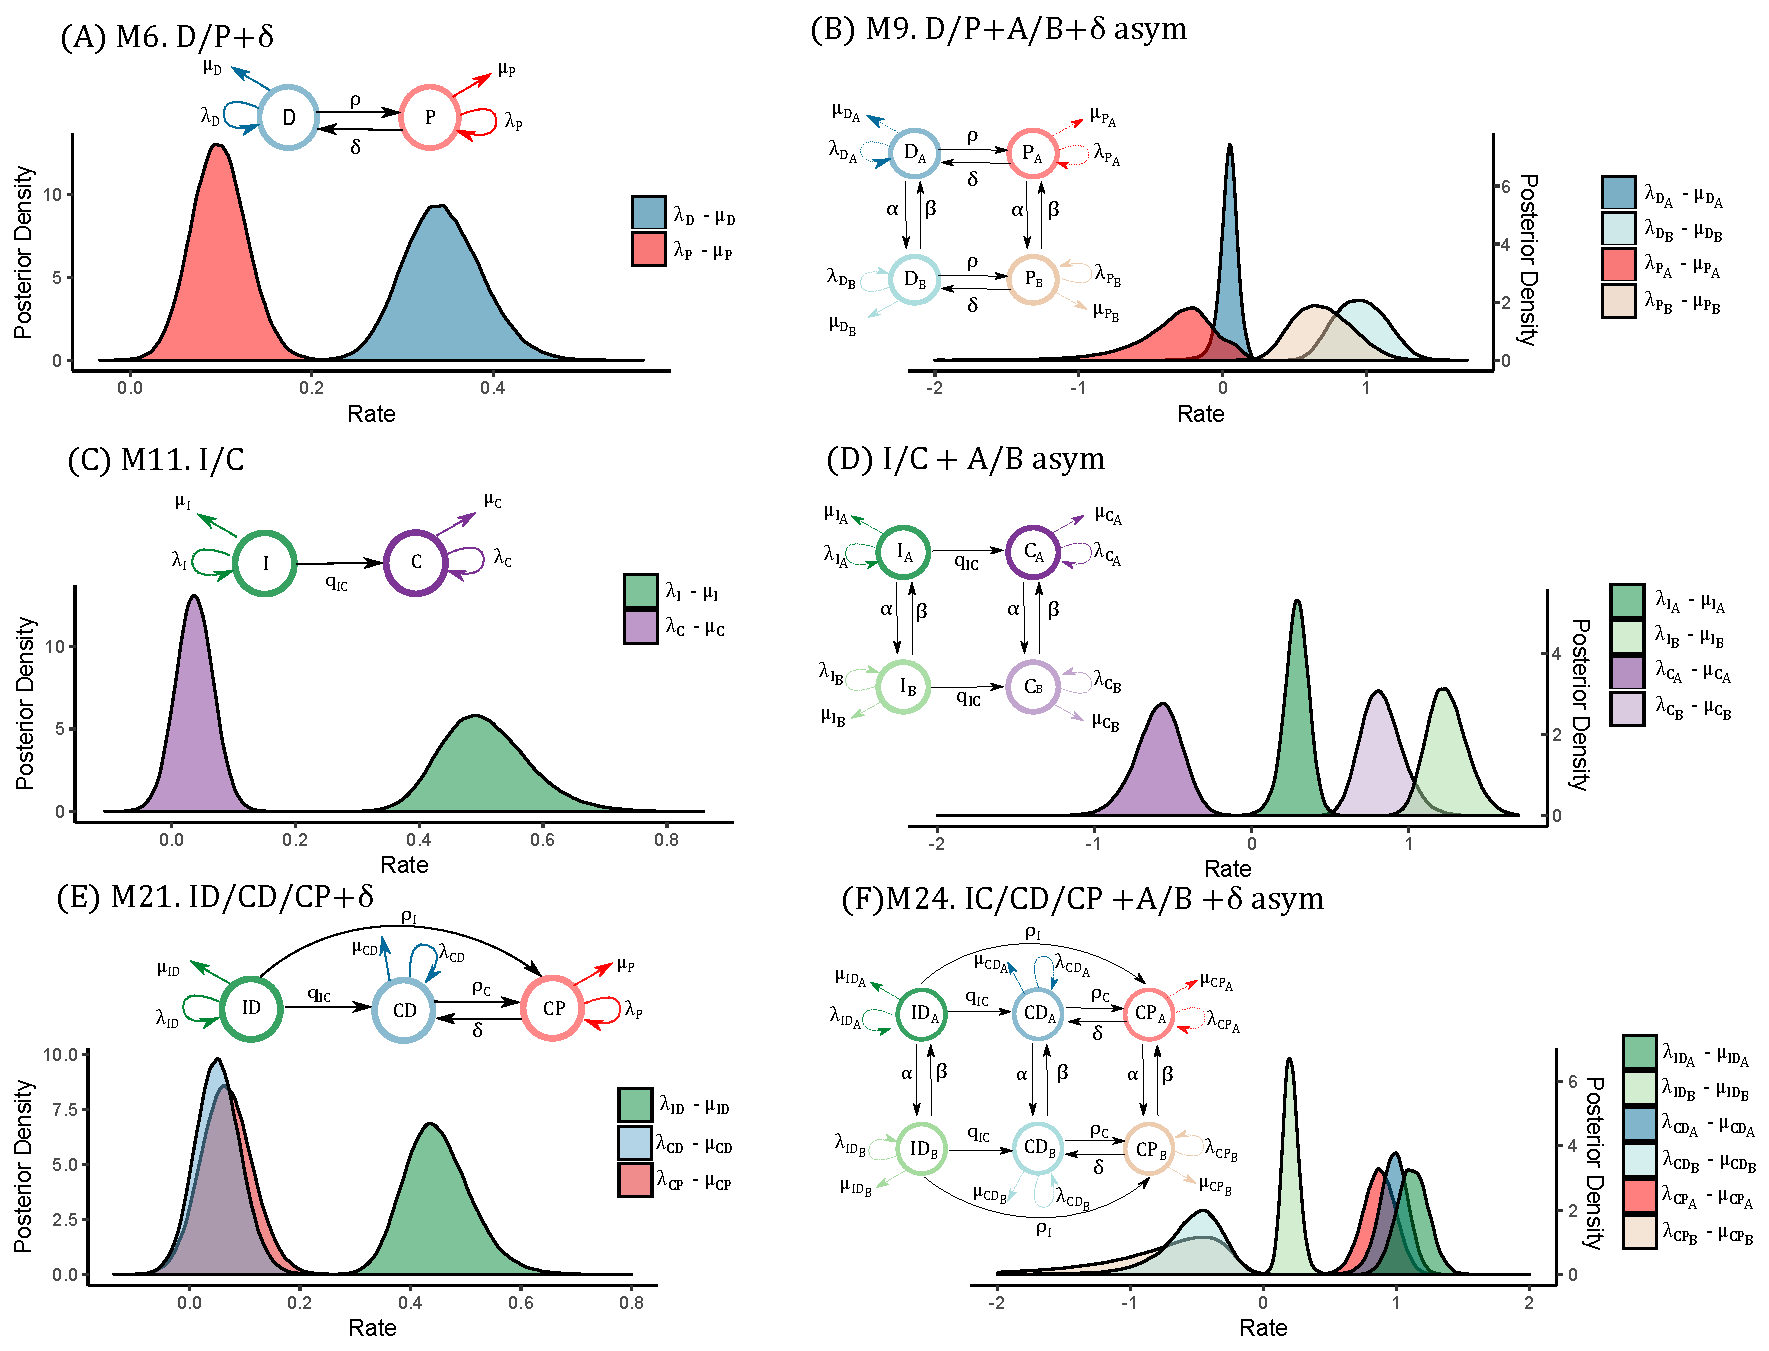
\includegraphics[width=\textwidth]{figS18.pdf}
\caption{Posterior distributions for the net diversification rates of the preferred models with diploidization. Red color represents diploid state $D$, blue color represents polyploid state $P$, green color represents self-incompatible $I$, purple color represents self-compatible $C$,  dark colors represent hidden state $A$ and light colors hidden state $B$.  (A) Ploidy only model M6. (B) Ploidy and hidden states model M9 (C) Breeding systems only model M11. (D) Breeding systems and hidden state model M14. (E) Ploidy and breeding systems model M21. (F) Ploidy, breeding systems, and hidden states model M24.} % XXX
\label{suppfigure:alldip}
\end{suppfigure}
